\documentclass[twoside]{book}

% Packages required by doxygen
\usepackage{fixltx2e}
\usepackage{calc}
\usepackage{doxygen}
\usepackage[export]{adjustbox} % also loads graphicx
\usepackage{graphicx}
\usepackage[utf8]{inputenc}
\usepackage{makeidx}
\usepackage{multicol}
\usepackage{multirow}
\PassOptionsToPackage{warn}{textcomp}
\usepackage{textcomp}
\usepackage[nointegrals]{wasysym}
\usepackage[table]{xcolor}

% Font selection
\usepackage[T1]{fontenc}
\usepackage[scaled=.90]{helvet}
\usepackage{courier}
\usepackage{amssymb}
\usepackage{sectsty}
\renewcommand{\familydefault}{\sfdefault}
\allsectionsfont{%
  \fontseries{bc}\selectfont%
  \color{darkgray}%
}
\renewcommand{\DoxyLabelFont}{%
  \fontseries{bc}\selectfont%
  \color{darkgray}%
}
\newcommand{\+}{\discretionary{\mbox{\scriptsize$\hookleftarrow$}}{}{}}

% Page & text layout
\usepackage{geometry}
\geometry{%
  a4paper,%
  top=2.5cm,%
  bottom=2.5cm,%
  left=2.5cm,%
  right=2.5cm%
}
\tolerance=750
\hfuzz=15pt
\hbadness=750
\setlength{\emergencystretch}{15pt}
\setlength{\parindent}{0cm}
\setlength{\parskip}{3ex plus 2ex minus 2ex}
\makeatletter
\renewcommand{\paragraph}{%
  \@startsection{paragraph}{4}{0ex}{-1.0ex}{1.0ex}{%
    \normalfont\normalsize\bfseries\SS@parafont%
  }%
}
\renewcommand{\subparagraph}{%
  \@startsection{subparagraph}{5}{0ex}{-1.0ex}{1.0ex}{%
    \normalfont\normalsize\bfseries\SS@subparafont%
  }%
}
\makeatother

% Headers & footers
\usepackage{fancyhdr}
\pagestyle{fancyplain}
\fancyhead[LE]{\fancyplain{}{\bfseries\thepage}}
\fancyhead[CE]{\fancyplain{}{}}
\fancyhead[RE]{\fancyplain{}{\bfseries\leftmark}}
\fancyhead[LO]{\fancyplain{}{\bfseries\rightmark}}
\fancyhead[CO]{\fancyplain{}{}}
\fancyhead[RO]{\fancyplain{}{\bfseries\thepage}}
\fancyfoot[LE]{\fancyplain{}{}}
\fancyfoot[CE]{\fancyplain{}{}}
\fancyfoot[RE]{\fancyplain{}{\bfseries\scriptsize Generated by Doxygen }}
\fancyfoot[LO]{\fancyplain{}{\bfseries\scriptsize Generated by Doxygen }}
\fancyfoot[CO]{\fancyplain{}{}}
\fancyfoot[RO]{\fancyplain{}{}}
\renewcommand{\footrulewidth}{0.4pt}
\renewcommand{\chaptermark}[1]{%
  \markboth{#1}{}%
}
\renewcommand{\sectionmark}[1]{%
  \markright{\thesection\ #1}%
}

% Indices & bibliography
\usepackage{natbib}
\usepackage[titles]{tocloft}
\setcounter{tocdepth}{3}
\setcounter{secnumdepth}{5}
\makeindex

% Custom commands
\newcommand{\clearemptydoublepage}{%
  \newpage{\pagestyle{empty}\cleardoublepage}%
}

\usepackage{caption}
\captionsetup{labelsep=space,justification=centering,font={bf},singlelinecheck=off,skip=4pt,position=top}

%===== C O N T E N T S =====

\begin{document}

% Titlepage & ToC
\pagenumbering{alph}
\begin{titlepage}
\vspace*{7cm}
\begin{center}%
{\Large Projekt2 }\\
\vspace*{1cm}
{\large Generated by Doxygen 1.8.13}\\
\end{center}
\end{titlepage}
\clearemptydoublepage
\pagenumbering{roman}
\tableofcontents
\clearemptydoublepage
\pagenumbering{arabic}

%--- Begin generated contents ---
\chapter{Hierarchical Index}
\section{Class Hierarchy}
This inheritance list is sorted roughly, but not completely, alphabetically\+:\begin{DoxyCompactList}
\item \contentsline{section}{Pojazd}{\pageref{class_pojazd}}{}
\begin{DoxyCompactList}
\item \contentsline{section}{Pociag}{\pageref{class_pociag}}{}
\begin{DoxyCompactList}
\item \contentsline{section}{Pociag\+Towarowy}{\pageref{class_pociag_towarowy}}{}
\end{DoxyCompactList}
\item \contentsline{section}{Samochod}{\pageref{class_samochod}}{}
\end{DoxyCompactList}
\item \contentsline{section}{Pracownik}{\pageref{class_pracownik}}{}
\item \contentsline{section}{Trasa}{\pageref{class_trasa}}{}
\item \contentsline{section}{Wagony}{\pageref{class_wagony}}{}
\end{DoxyCompactList}

\chapter{Class Index}
\section{Class List}
Here are the classes, structs, unions and interfaces with brief descriptions\+:\begin{DoxyCompactList}
\item\contentsline{section}{\textbf{ Pociag} \\*Klasa Pociąg, pochodna klasy \doxyref{Pojazd}{p.}{class_pojazd} }{\pageref{class_pociag}}{}
\item\contentsline{section}{\textbf{ Pociag\+Towarowy} \\*Klasa \doxyref{Pociag\+Towarowy}{p.}{class_pociag_towarowy}, pochodna klasy \doxyref{Pociag}{p.}{class_pociag} }{\pageref{class_pociag_towarowy}}{}
\item\contentsline{section}{\textbf{ Pojazd} \\*Klasa abstrakcyjna }{\pageref{class_pojazd}}{}
\item\contentsline{section}{\textbf{ Pracownik} \\*Klasa \doxyref{Pracownik}{p.}{class_pracownik}, podklasa klasy \doxyref{Pociag}{p.}{class_pociag} }{\pageref{class_pracownik}}{}
\item\contentsline{section}{\textbf{ Samochod} \\*Klasa \doxyref{Samochod}{p.}{class_samochod}, pochodna klasy \doxyref{Pojazd}{p.}{class_pojazd} }{\pageref{class_samochod}}{}
\item\contentsline{section}{\textbf{ Trasa} \\*Klasa \doxyref{Trasa}{p.}{class_trasa}, podklasa klasy \doxyref{Pociag}{p.}{class_pociag} }{\pageref{class_trasa}}{}
\item\contentsline{section}{\textbf{ Wagony} \\*Klasa \doxyref{Wagony}{p.}{class_wagony}, podklasa klasy \doxyref{Pociag}{p.}{class_pociag} }{\pageref{class_wagony}}{}
\end{DoxyCompactList}

\chapter{File Index}
\section{File List}
Here is a list of all files with brief descriptions\+:\begin{DoxyCompactList}
\item\contentsline{section}{\textbf{ Pociag towarowy.\+cpp} }{\pageref{_pociag_01towarowy_8cpp}}{}
\item\contentsline{section}{\textbf{ Pociag towarowy.\+h} }{\pageref{_pociag_01towarowy_8h}}{}
\item\contentsline{section}{\textbf{ pociag.\+cpp} }{\pageref{pociag_8cpp}}{}
\item\contentsline{section}{\textbf{ pociag.\+h} }{\pageref{pociag_8h}}{}
\item\contentsline{section}{\textbf{ Pojazd.\+cpp} }{\pageref{_pojazd_8cpp}}{}
\item\contentsline{section}{\textbf{ Pojazd.\+h} }{\pageref{_pojazd_8h}}{}
\item\contentsline{section}{\textbf{ pracownik.\+cpp} }{\pageref{pracownik_8cpp}}{}
\item\contentsline{section}{\textbf{ pracownik.\+h} }{\pageref{pracownik_8h}}{}
\item\contentsline{section}{\textbf{ P\+R\+O\+J\+E\+K\+T.\+cpp} }{\pageref{_p_r_o_j_e_k_t_8cpp}}{}
\item\contentsline{section}{\textbf{ Samochód.\+cpp} }{\pageref{_samoch_xC3_xB3d_8cpp}}{}
\item\contentsline{section}{\textbf{ Samochód.\+h} }{\pageref{_samoch_xC3_xB3d_8h}}{}
\item\contentsline{section}{\textbf{ stdafx.\+cpp} }{\pageref{stdafx_8cpp}}{}
\item\contentsline{section}{\textbf{ stdafx.\+h} }{\pageref{stdafx_8h}}{}
\item\contentsline{section}{\textbf{ targetver.\+h} }{\pageref{targetver_8h}}{}
\item\contentsline{section}{\textbf{ trasa.\+cpp} }{\pageref{trasa_8cpp}}{}
\item\contentsline{section}{\textbf{ trasa.\+h} }{\pageref{trasa_8h}}{}
\item\contentsline{section}{\textbf{ wagony.\+cpp} }{\pageref{wagony_8cpp}}{}
\item\contentsline{section}{\textbf{ wagony.\+h} }{\pageref{wagony_8h}}{}
\end{DoxyCompactList}

\chapter{Class Documentation}
\section{Pociag Class Reference}
\label{class_pociag}\index{Pociag@{Pociag}}


Klasa Pociąg, pochodna klasy \doxyref{Pojazd}{p.}{class_pojazd}.  




{\ttfamily \#include $<$pociag.\+h$>$}

Inheritance diagram for Pociag\+:\begin{figure}[H]
\begin{center}
\leavevmode
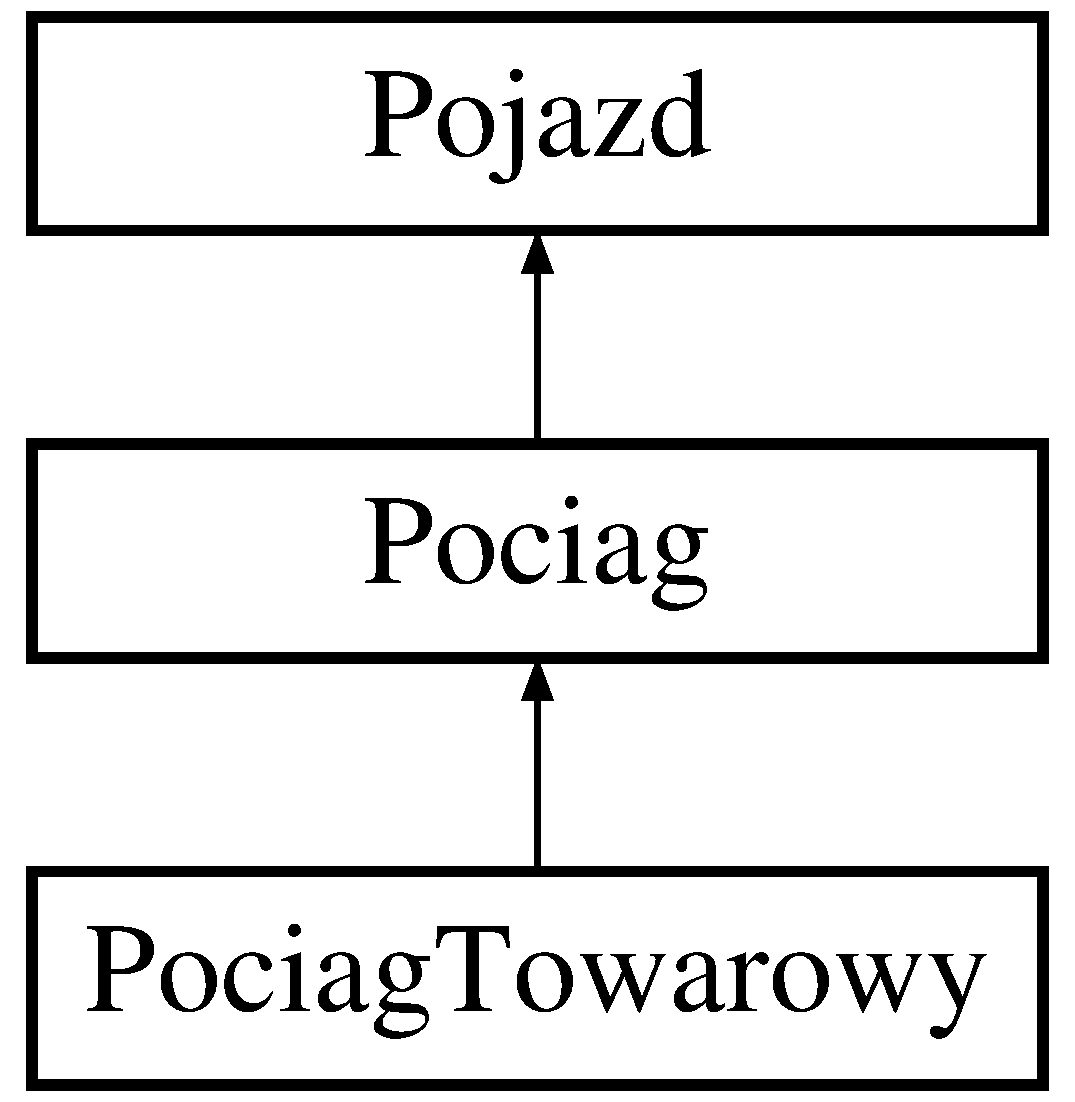
\includegraphics[height=3.000000cm]{class_pociag}
\end{center}
\end{figure}
\subsection*{Public Member Functions}
\begin{DoxyCompactItemize}
\item 
\textbf{ Pociag} ()
\begin{DoxyCompactList}\small\item\em Konstruktor domyślny. \end{DoxyCompactList}\item 
\textbf{ Pociag} (string nazwa\+\_\+p, int \textbf{ rok\+\_\+produkcji}, string \textbf{ kolor}, int liczba\+\_\+w, string poczatek\+\_\+t, string koniec\+\_\+t, int czas\+\_\+przejazdu, int dlugosc\+\_\+t)
\item 
\textbf{ $\sim$\+Pociag} ()
\begin{DoxyCompactList}\small\item\em Destruktor. \end{DoxyCompactList}\item 
\textbf{ Pociag} (const \textbf{ Pociag} \&pociag)
\begin{DoxyCompactList}\small\item\em Konstruktor kopiujący. \end{DoxyCompactList}\item 
void \textbf{ wyswietl\+Dane} ()
\begin{DoxyCompactList}\small\item\em Funkcja wirtualna wyświetlająca dane pociągu. \end{DoxyCompactList}\item 
void \textbf{ dodaj\+Dane\+Pociagu} (string nazwa\+\_\+p, int \textbf{ rok\+\_\+produkcji}, string kolor\+\_\+p, int liczba\+\_\+w, string poczatek\+\_\+t, string koniec\+\_\+t, int czas\+\_\+przejazdu, int dlugosc\+\_\+t)
\item 
void \textbf{ zmien\+Nazwe} (string nowa\+\_\+nazwa)
\item 
void \textbf{ dodaj\+Pracownika} (string nowy\+\_\+imie\+\_\+nazwisko, string nowy\+\_\+zawod, int nowy\+\_\+zarobki)
\item 
void \textbf{ dodaj\+Wagony\+Pociagu} (int ile\+\_\+wagonow\+\_\+pociagu)
\item 
void \textbf{ zmien\+Kolor\+Wagonow} (string nowy\+\_\+kolor\+\_\+wagonow)
\item 
void \textbf{ zmien\+Kolor} (string nowy\+\_\+kolor\+\_\+pocigu)
\item 
void \textbf{ zapisz} (\textbf{ Pociag} \&pociag)
\item 
void \textbf{ wczytaj} (\textbf{ Pociag} \&pociag)
\item 
bool \textbf{ operator==} (const \textbf{ Pociag} \&p)
\begin{DoxyCompactList}\small\item\em Operator ==. \end{DoxyCompactList}\item 
bool \textbf{ operator$>$} (const \textbf{ Pociag} \&p)
\begin{DoxyCompactList}\small\item\em Operator $>$ \end{DoxyCompactList}\item 
bool \textbf{ operator$<$} (const \textbf{ Pociag} \&p)
\begin{DoxyCompactList}\small\item\em Operator $<$. \end{DoxyCompactList}\item 
\textbf{ Pociag} \& \textbf{ operator=} (const \textbf{ Pociag} \&p)
\begin{DoxyCompactList}\small\item\em Operator =. \end{DoxyCompactList}\item 
\textbf{ Pociag} \textbf{ operator+} (const \textbf{ Pociag} \&p)
\begin{DoxyCompactList}\small\item\em Operator+. \end{DoxyCompactList}\item 
\textbf{ Pociag} \& \textbf{ operator++} (int)
\begin{DoxyCompactList}\small\item\em Operator ++. \end{DoxyCompactList}\item 
\textbf{ Pociag} \& \textbf{ operator-\/-\/} (int)
\begin{DoxyCompactList}\small\item\em Operator --. \end{DoxyCompactList}\item 
\textbf{ Pracownik} \& \textbf{ operator[$\,$]} (int i)
\begin{DoxyCompactList}\small\item\em Operator indeksowy. \end{DoxyCompactList}\item 
\textbf{ operator int} ()
\begin{DoxyCompactList}\small\item\em Operator rzutowania. \end{DoxyCompactList}\end{DoxyCompactItemize}
\subsection*{Static Public Member Functions}
\begin{DoxyCompactItemize}
\item 
static int \textbf{ wyswietl\+Liczbe\+Pociagow} ()
\begin{DoxyCompactList}\small\item\em metoda statyczna zwracająca liczbe pociągów \end{DoxyCompactList}\end{DoxyCompactItemize}
\subsection*{Protected Attributes}
\begin{DoxyCompactItemize}
\item 
string \textbf{ nazwa\+\_\+pociagu}
\begin{DoxyCompactList}\small\item\em określa nazwe pociągu \end{DoxyCompactList}\item 
int \textbf{ liczba\+\_\+pracownikow}
\begin{DoxyCompactList}\small\item\em określa liczbę pracowników w pociągu \end{DoxyCompactList}\item 
\textbf{ Wagony} \textbf{ wagony}
\begin{DoxyCompactList}\small\item\em określa wagony pociągu \end{DoxyCompactList}\item 
vector$<$ \textbf{ Pracownik} $>$ \textbf{ pracownicy}
\begin{DoxyCompactList}\small\item\em określa pracowników pociągu \end{DoxyCompactList}\item 
\textbf{ Trasa} \textbf{ trasa}
\begin{DoxyCompactList}\small\item\em określa trase pociągu \end{DoxyCompactList}\end{DoxyCompactItemize}
\subsection*{Static Protected Attributes}
\begin{DoxyCompactItemize}
\item 
static int \textbf{ ilosc\+\_\+pociagow} = 0
\begin{DoxyCompactList}\small\item\em zmienna statyczna przechowująca ilość pociągów \end{DoxyCompactList}\end{DoxyCompactItemize}
\subsection*{Friends}
\begin{DoxyCompactItemize}
\item 
ostream \& \textbf{ operator$<$$<$} (ostream \&s, \textbf{ Pociag} \&p)
\begin{DoxyCompactList}\small\item\em operator strumieniowy $<$$<$ \end{DoxyCompactList}\item 
istream \& \textbf{ operator$>$$>$} (istream \&s, \textbf{ Pociag} \&p)
\begin{DoxyCompactList}\small\item\em operator strumieniowy $>$$>$ \end{DoxyCompactList}\end{DoxyCompactItemize}


\subsection{Detailed Description}
Klasa Pociąg, pochodna klasy \doxyref{Pojazd}{p.}{class_pojazd}. 

\subsection{Constructor \& Destructor Documentation}
\mbox{\label{class_pociag_aa09d236a07401ce066854498eba23712}} 
\index{Pociag@{Pociag}!Pociag@{Pociag}}
\index{Pociag@{Pociag}!Pociag@{Pociag}}
\subsubsection{Pociag()\hspace{0.1cm}{\footnotesize\ttfamily [1/3]}}
{\footnotesize\ttfamily Pociag\+::\+Pociag (\begin{DoxyParamCaption}{ }\end{DoxyParamCaption})}



Konstruktor domyślny. 

\mbox{\label{class_pociag_a938af7820cab214b07ce520366663074}} 
\index{Pociag@{Pociag}!Pociag@{Pociag}}
\index{Pociag@{Pociag}!Pociag@{Pociag}}
\subsubsection{Pociag()\hspace{0.1cm}{\footnotesize\ttfamily [2/3]}}
{\footnotesize\ttfamily Pociag\+::\+Pociag (\begin{DoxyParamCaption}\item[{string}]{nazwa\+\_\+p,  }\item[{int}]{rok\+\_\+produkcji,  }\item[{string}]{kolor,  }\item[{int}]{liczba\+\_\+w,  }\item[{string}]{poczatek\+\_\+t,  }\item[{string}]{koniec\+\_\+t,  }\item[{int}]{czas\+\_\+przejazdu,  }\item[{int}]{dlugosc\+\_\+t }\end{DoxyParamCaption})}

Konstruktor Jako parametry przyjmuje nową nazwę pociągu, nowy rok produkcji pociągu nowy kolor,nową liczbę wagonów, nowy początek trasy pociągu, nowy koniec trasy pociągu, nowy czas przejazdu pociągu, nową długość trasy w kilometrach 
\begin{DoxyParams}{Parameters}
{\em nazwa\+\_\+p} & określa nazwę pociągu \\
\hline
{\em rok\+\_\+produkcji} & określa rok produkcji pociągu \\
\hline
{\em } & \\
\hline
\end{DoxyParams}
\mbox{\label{class_pociag_ae45cf91403955fd03ac41ae7c295b4a9}} 
\index{Pociag@{Pociag}!````~Pociag@{$\sim$\+Pociag}}
\index{````~Pociag@{$\sim$\+Pociag}!Pociag@{Pociag}}
\subsubsection{$\sim$\+Pociag()}
{\footnotesize\ttfamily Pociag\+::$\sim$\+Pociag (\begin{DoxyParamCaption}{ }\end{DoxyParamCaption})}



Destruktor. 

\mbox{\label{class_pociag_aa01d38fb2548b217ae793f32795fb835}} 
\index{Pociag@{Pociag}!Pociag@{Pociag}}
\index{Pociag@{Pociag}!Pociag@{Pociag}}
\subsubsection{Pociag()\hspace{0.1cm}{\footnotesize\ttfamily [3/3]}}
{\footnotesize\ttfamily Pociag\+::\+Pociag (\begin{DoxyParamCaption}\item[{const \textbf{ Pociag} \&}]{pociag }\end{DoxyParamCaption})}



Konstruktor kopiujący. 



\subsection{Member Function Documentation}
\mbox{\label{class_pociag_aea1241109c8a6ea3cc8a4cd433021e41}} 
\index{Pociag@{Pociag}!dodaj\+Dane\+Pociagu@{dodaj\+Dane\+Pociagu}}
\index{dodaj\+Dane\+Pociagu@{dodaj\+Dane\+Pociagu}!Pociag@{Pociag}}
\subsubsection{dodaj\+Dane\+Pociagu()}
{\footnotesize\ttfamily void Pociag\+::dodaj\+Dane\+Pociagu (\begin{DoxyParamCaption}\item[{string}]{nazwa\+\_\+p,  }\item[{int}]{rok\+\_\+produkcji,  }\item[{string}]{kolor\+\_\+p,  }\item[{int}]{liczba\+\_\+w,  }\item[{string}]{poczatek\+\_\+t,  }\item[{string}]{koniec\+\_\+t,  }\item[{int}]{czas\+\_\+przejazdu,  }\item[{int}]{dlugosc\+\_\+t }\end{DoxyParamCaption})}

Procedura zmieniająca dane pociągu. Jako parametry przyjmuje nową nazwę pociągu, nowy rok produkcji pociągu,nowy kolor pociągu, nową liczbę wagonów, nowy początek trasy pociągu, nowy koniec trasy pociągu, nowy czas przejazdu pociągu, nową długość trasy w kilometrach 
\begin{DoxyParams}{Parameters}
{\em nazwa\+\_\+p} & określa nazwę pociągu \\
\hline
{\em rok\+\_\+produkcji} & określa rok produkcji pociągu \\
\hline
{\em kolor\+\_\+p} & określa nowy kolor pociągu \\
\hline
{\em liczba\+\_\+w} & określa liczbę wagonów \\
\hline
{\em poczatek\+\_\+t} & określa początek trasy pociągu \\
\hline
{\em koniec\+\_\+t} & określa koniec trasy pociągu \\
\hline
{\em czas\+\_\+przejazdu} & określa czas przejazdu pociągu \\
\hline
{\em dlugosc\+\_\+t} & określa długość trasy w kilometrach \\
\hline
\end{DoxyParams}
\begin{DoxyReturn}{Returns}
Funkcja nie zwraca żadnej wartości 
\end{DoxyReturn}
\mbox{\label{class_pociag_af4eadc978c7779c832da7ad4fe2bc86f}} 
\index{Pociag@{Pociag}!dodaj\+Pracownika@{dodaj\+Pracownika}}
\index{dodaj\+Pracownika@{dodaj\+Pracownika}!Pociag@{Pociag}}
\subsubsection{dodaj\+Pracownika()}
{\footnotesize\ttfamily void Pociag\+::dodaj\+Pracownika (\begin{DoxyParamCaption}\item[{string}]{nowy\+\_\+imie\+\_\+nazwisko,  }\item[{string}]{nowy\+\_\+zawod,  }\item[{int}]{nowy\+\_\+zarobki }\end{DoxyParamCaption})}

Funkcja dodająca pracownika. Jako parametry podawane są\+: imię i nazwisko, zawód, zarobki 
\begin{DoxyParams}{Parameters}
{\em nowy\+\_\+imie\+\_\+nazwisko} & określa imie i nazwisko pracownika \\
\hline
{\em nowy\+\_\+zawod} & określa zawód pracownika \\
\hline
{\em nowy\+\_\+zarobki} & określa zarobki pracownika \\
\hline
\end{DoxyParams}
\begin{DoxyReturn}{Returns}
Funkcja nie zwraca żadnej wartości 
\end{DoxyReturn}
\mbox{\label{class_pociag_ae0f8e4d7f079baf9ac4f72688cc414e3}} 
\index{Pociag@{Pociag}!dodaj\+Wagony\+Pociagu@{dodaj\+Wagony\+Pociagu}}
\index{dodaj\+Wagony\+Pociagu@{dodaj\+Wagony\+Pociagu}!Pociag@{Pociag}}
\subsubsection{dodaj\+Wagony\+Pociagu()}
{\footnotesize\ttfamily void Pociag\+::dodaj\+Wagony\+Pociagu (\begin{DoxyParamCaption}\item[{int}]{ile\+\_\+wagonow\+\_\+pociagu }\end{DoxyParamCaption})}

Funckcja dodająca wagony do pociągu. Jako parametr podawana jest liczba wagonów, które chce sie dołączyć do pojazdu 
\begin{DoxyParams}{Parameters}
{\em ile\+\_\+wagonow\+\_\+pociagu} & określa liczbe wagonów \\
\hline
\end{DoxyParams}
\begin{DoxyReturn}{Returns}
Funkcja nie zwraca żadnej wartości 
\end{DoxyReturn}
\mbox{\label{class_pociag_a358e8b9db75dd92378892f2df39cf4bf}} 
\index{Pociag@{Pociag}!operator int@{operator int}}
\index{operator int@{operator int}!Pociag@{Pociag}}
\subsubsection{operator int()}
{\footnotesize\ttfamily Pociag\+::operator int (\begin{DoxyParamCaption}{ }\end{DoxyParamCaption})}



Operator rzutowania. 

\begin{DoxyReturn}{Returns}
Zwraca liczbe pracowników pociągu 
\end{DoxyReturn}
\mbox{\label{class_pociag_a172506e48bebd907ef5a8fb5f78347e2}} 
\index{Pociag@{Pociag}!operator+@{operator+}}
\index{operator+@{operator+}!Pociag@{Pociag}}
\subsubsection{operator+()}
{\footnotesize\ttfamily \textbf{ Pociag} Pociag\+::operator+ (\begin{DoxyParamCaption}\item[{const \textbf{ Pociag} \&}]{p }\end{DoxyParamCaption})}



Operator+. 

\mbox{\label{class_pociag_a4d9a774fa5595057108c11795e01b2fd}} 
\index{Pociag@{Pociag}!operator++@{operator++}}
\index{operator++@{operator++}!Pociag@{Pociag}}
\subsubsection{operator++()}
{\footnotesize\ttfamily \textbf{ Pociag} \& Pociag\+::operator++ (\begin{DoxyParamCaption}\item[{int}]{ }\end{DoxyParamCaption})}



Operator ++. 

\mbox{\label{class_pociag_afec73939f666119863b4b10f2bf64c34}} 
\index{Pociag@{Pociag}!operator-\/-\/@{operator-\/-\/}}
\index{operator-\/-\/@{operator-\/-\/}!Pociag@{Pociag}}
\subsubsection{operator-\/-\/()}
{\footnotesize\ttfamily \textbf{ Pociag} \& Pociag\+::operator-\/-\/ (\begin{DoxyParamCaption}\item[{int}]{ }\end{DoxyParamCaption})}



Operator --. 

\mbox{\label{class_pociag_a8c6e9316d42b86dfb627c30a9ab1a771}} 
\index{Pociag@{Pociag}!operator$<$@{operator$<$}}
\index{operator$<$@{operator$<$}!Pociag@{Pociag}}
\subsubsection{operator$<$()}
{\footnotesize\ttfamily bool Pociag\+::operator$<$ (\begin{DoxyParamCaption}\item[{const \textbf{ Pociag} \&}]{p }\end{DoxyParamCaption})}



Operator $<$. 

\mbox{\label{class_pociag_afe13aa599592fc51dab54f1faefbcd89}} 
\index{Pociag@{Pociag}!operator=@{operator=}}
\index{operator=@{operator=}!Pociag@{Pociag}}
\subsubsection{operator=()}
{\footnotesize\ttfamily \textbf{ Pociag} \& Pociag\+::operator= (\begin{DoxyParamCaption}\item[{const \textbf{ Pociag} \&}]{p }\end{DoxyParamCaption})}



Operator =. 

\mbox{\label{class_pociag_aaeaf319bfca975314c3b9413423180aa}} 
\index{Pociag@{Pociag}!operator==@{operator==}}
\index{operator==@{operator==}!Pociag@{Pociag}}
\subsubsection{operator==()}
{\footnotesize\ttfamily bool Pociag\+::operator== (\begin{DoxyParamCaption}\item[{const \textbf{ Pociag} \&}]{p }\end{DoxyParamCaption})}



Operator ==. 

\mbox{\label{class_pociag_a5b1746f109f0baf0ee68ca3e9ef2ef37}} 
\index{Pociag@{Pociag}!operator$>$@{operator$>$}}
\index{operator$>$@{operator$>$}!Pociag@{Pociag}}
\subsubsection{operator$>$()}
{\footnotesize\ttfamily bool Pociag\+::operator$>$ (\begin{DoxyParamCaption}\item[{const \textbf{ Pociag} \&}]{p }\end{DoxyParamCaption})}



Operator $>$ 

\mbox{\label{class_pociag_aff28f36ce1d39a760b0b5da595921f4a}} 
\index{Pociag@{Pociag}!operator[]@{operator[]}}
\index{operator[]@{operator[]}!Pociag@{Pociag}}
\subsubsection{operator[]()}
{\footnotesize\ttfamily \textbf{ Pracownik} \& Pociag\+::operator[$\,$] (\begin{DoxyParamCaption}\item[{int}]{i }\end{DoxyParamCaption})}



Operator indeksowy. 


\begin{DoxyParams}{Parameters}
{\em i} & oznacza numer pracownika \\
\hline
\end{DoxyParams}
\begin{DoxyReturn}{Returns}
Zwraca pracownika o danym numerze 
\end{DoxyReturn}
\mbox{\label{class_pociag_adbcfb0b338e89e19e148e3aa97ba3fe5}} 
\index{Pociag@{Pociag}!wczytaj@{wczytaj}}
\index{wczytaj@{wczytaj}!Pociag@{Pociag}}
\subsubsection{wczytaj()}
{\footnotesize\ttfamily void Pociag\+::wczytaj (\begin{DoxyParamCaption}\item[{\textbf{ Pociag} \&}]{pociag }\end{DoxyParamCaption})}

Funkcja wczytująca obiekt z pliku Jako parametr przyjmuje obiekt pociąg i wczytuje do niego informacje z pliku 
\begin{DoxyParams}{Parameters}
{\em pociag} & określa pociag do którego wczytujemy dane \\
\hline
\end{DoxyParams}
\mbox{\label{class_pociag_a1096a05d2981c1da0ac50870d37c1ffb}} 
\index{Pociag@{Pociag}!wyswietl\+Dane@{wyswietl\+Dane}}
\index{wyswietl\+Dane@{wyswietl\+Dane}!Pociag@{Pociag}}
\subsubsection{wyswietl\+Dane()}
{\footnotesize\ttfamily void Pociag\+::wyswietl\+Dane (\begin{DoxyParamCaption}{ }\end{DoxyParamCaption})\hspace{0.3cm}{\ttfamily [virtual]}}



Funkcja wirtualna wyświetlająca dane pociągu. 



Implements \textbf{ Pojazd} \doxyref{}{p.}{class_pojazd_a945485210fbea0be179644bd68863304}.

\mbox{\label{class_pociag_a30c319e65a8d40e36925ba16a44700bb}} 
\index{Pociag@{Pociag}!wyswietl\+Liczbe\+Pociagow@{wyswietl\+Liczbe\+Pociagow}}
\index{wyswietl\+Liczbe\+Pociagow@{wyswietl\+Liczbe\+Pociagow}!Pociag@{Pociag}}
\subsubsection{wyswietl\+Liczbe\+Pociagow()}
{\footnotesize\ttfamily static int Pociag\+::wyswietl\+Liczbe\+Pociagow (\begin{DoxyParamCaption}{ }\end{DoxyParamCaption})\hspace{0.3cm}{\ttfamily [inline]}, {\ttfamily [static]}}



metoda statyczna zwracająca liczbe pociągów 

\mbox{\label{class_pociag_a49faf5fc94d3622ce3ce9717e4f0de3b}} 
\index{Pociag@{Pociag}!zapisz@{zapisz}}
\index{zapisz@{zapisz}!Pociag@{Pociag}}
\subsubsection{zapisz()}
{\footnotesize\ttfamily void Pociag\+::zapisz (\begin{DoxyParamCaption}\item[{\textbf{ Pociag} \&}]{pociag }\end{DoxyParamCaption})}

Funkcja zapisująca pociąg do pliku Jako parametr przyjmuje obiekt pociąg i zapisuje informacje o nim do pliku 
\begin{DoxyParams}{Parameters}
{\em pociag} & określa pociag którego dane zapisujemy \\
\hline
\end{DoxyParams}
\mbox{\label{class_pociag_a5645f7c8f4019124e63e41444b6893b4}} 
\index{Pociag@{Pociag}!zmien\+Kolor@{zmien\+Kolor}}
\index{zmien\+Kolor@{zmien\+Kolor}!Pociag@{Pociag}}
\subsubsection{zmien\+Kolor()}
{\footnotesize\ttfamily void Pociag\+::zmien\+Kolor (\begin{DoxyParamCaption}\item[{string}]{nowy\+\_\+kolor\+\_\+pocigu }\end{DoxyParamCaption})\hspace{0.3cm}{\ttfamily [virtual]}}

Funckcja wirtualna zmieniająca kolor pociągu . Jako parametr podawany jest nowy kolor pociągu /param nowy\+\_\+kolor określa kolor pociągu /return Funkcja nie zwraca żadnej wartości 

Implements \textbf{ Pojazd} \doxyref{}{p.}{class_pojazd_a29cab7cc8f5b4b3faed884f0d2849f4f}.

\mbox{\label{class_pociag_a02e5effbee4eb32de3e1099a72e1cba0}} 
\index{Pociag@{Pociag}!zmien\+Kolor\+Wagonow@{zmien\+Kolor\+Wagonow}}
\index{zmien\+Kolor\+Wagonow@{zmien\+Kolor\+Wagonow}!Pociag@{Pociag}}
\subsubsection{zmien\+Kolor\+Wagonow()}
{\footnotesize\ttfamily void Pociag\+::zmien\+Kolor\+Wagonow (\begin{DoxyParamCaption}\item[{string}]{nowy\+\_\+kolor\+\_\+wagonow }\end{DoxyParamCaption})}

Funckcja zmieniająca kolor wagonów . Jako parametr podawany jest nowy kolor wagonów 
\begin{DoxyParams}{Parameters}
{\em nowy\+\_\+kolor\+\_\+wagonow} & określa kolor wagonów \\
\hline
\end{DoxyParams}
\begin{DoxyReturn}{Returns}
Funkcja nie zwraca żadnej wartości 
\end{DoxyReturn}
\mbox{\label{class_pociag_a6c0758995a78c594f122201c949ae06c}} 
\index{Pociag@{Pociag}!zmien\+Nazwe@{zmien\+Nazwe}}
\index{zmien\+Nazwe@{zmien\+Nazwe}!Pociag@{Pociag}}
\subsubsection{zmien\+Nazwe()}
{\footnotesize\ttfamily void Pociag\+::zmien\+Nazwe (\begin{DoxyParamCaption}\item[{string}]{nowa\+\_\+nazwa }\end{DoxyParamCaption})}

Funkcja zmieniająca nazwe pociągu. Przyjmuje jako parametr nową nazwe pociągu 
\begin{DoxyParams}{Parameters}
{\em nowa\+\_\+nazwa} & określa nazwę pociągu \\
\hline
\end{DoxyParams}
\begin{DoxyReturn}{Returns}
Funkcja nie zwraca żadnej wartości 
\end{DoxyReturn}


\subsection{Friends And Related Function Documentation}
\mbox{\label{class_pociag_aa69694c17cdb3e184cc54938668f705c}} 
\index{Pociag@{Pociag}!operator$<$$<$@{operator$<$$<$}}
\index{operator$<$$<$@{operator$<$$<$}!Pociag@{Pociag}}
\subsubsection{operator$<$$<$}
{\footnotesize\ttfamily ostream\& operator$<$$<$ (\begin{DoxyParamCaption}\item[{ostream \&}]{s,  }\item[{\textbf{ Pociag} \&}]{p }\end{DoxyParamCaption})\hspace{0.3cm}{\ttfamily [friend]}}



operator strumieniowy $<$$<$ 

\mbox{\label{class_pociag_a00926731077d7f0d7c1a81c50bee727d}} 
\index{Pociag@{Pociag}!operator$>$$>$@{operator$>$$>$}}
\index{operator$>$$>$@{operator$>$$>$}!Pociag@{Pociag}}
\subsubsection{operator$>$$>$}
{\footnotesize\ttfamily istream\& operator$>$$>$ (\begin{DoxyParamCaption}\item[{istream \&}]{s,  }\item[{\textbf{ Pociag} \&}]{p }\end{DoxyParamCaption})\hspace{0.3cm}{\ttfamily [friend]}}



operator strumieniowy $>$$>$ 



\subsection{Member Data Documentation}
\mbox{\label{class_pociag_aeb03002f5b8d01ba963c52ed9f946159}} 
\index{Pociag@{Pociag}!ilosc\+\_\+pociagow@{ilosc\+\_\+pociagow}}
\index{ilosc\+\_\+pociagow@{ilosc\+\_\+pociagow}!Pociag@{Pociag}}
\subsubsection{ilosc\+\_\+pociagow}
{\footnotesize\ttfamily int Pociag\+::ilosc\+\_\+pociagow = 0\hspace{0.3cm}{\ttfamily [static]}, {\ttfamily [protected]}}



zmienna statyczna przechowująca ilość pociągów 

\mbox{\label{class_pociag_a15c6cf934080b502f2d8d85643eb8e85}} 
\index{Pociag@{Pociag}!liczba\+\_\+pracownikow@{liczba\+\_\+pracownikow}}
\index{liczba\+\_\+pracownikow@{liczba\+\_\+pracownikow}!Pociag@{Pociag}}
\subsubsection{liczba\+\_\+pracownikow}
{\footnotesize\ttfamily int Pociag\+::liczba\+\_\+pracownikow\hspace{0.3cm}{\ttfamily [protected]}}



określa liczbę pracowników w pociągu 

\mbox{\label{class_pociag_a17321807df7ca8a8808b9845bec610e4}} 
\index{Pociag@{Pociag}!nazwa\+\_\+pociagu@{nazwa\+\_\+pociagu}}
\index{nazwa\+\_\+pociagu@{nazwa\+\_\+pociagu}!Pociag@{Pociag}}
\subsubsection{nazwa\+\_\+pociagu}
{\footnotesize\ttfamily string Pociag\+::nazwa\+\_\+pociagu\hspace{0.3cm}{\ttfamily [protected]}}



określa nazwe pociągu 

\mbox{\label{class_pociag_a0923922692ae0fdc2ed0f2bfcda7d4ce}} 
\index{Pociag@{Pociag}!pracownicy@{pracownicy}}
\index{pracownicy@{pracownicy}!Pociag@{Pociag}}
\subsubsection{pracownicy}
{\footnotesize\ttfamily vector$<$\textbf{ Pracownik}$>$ Pociag\+::pracownicy\hspace{0.3cm}{\ttfamily [protected]}}



określa pracowników pociągu 

\mbox{\label{class_pociag_aae7aabee2f3686fab558e429eac759db}} 
\index{Pociag@{Pociag}!trasa@{trasa}}
\index{trasa@{trasa}!Pociag@{Pociag}}
\subsubsection{trasa}
{\footnotesize\ttfamily \textbf{ Trasa} Pociag\+::trasa\hspace{0.3cm}{\ttfamily [protected]}}



określa trase pociągu 

\mbox{\label{class_pociag_aa54c466523b8bf15b1b7d63fbe37a955}} 
\index{Pociag@{Pociag}!wagony@{wagony}}
\index{wagony@{wagony}!Pociag@{Pociag}}
\subsubsection{wagony}
{\footnotesize\ttfamily \textbf{ Wagony} Pociag\+::wagony\hspace{0.3cm}{\ttfamily [protected]}}



określa wagony pociągu 



The documentation for this class was generated from the following files\+:\begin{DoxyCompactItemize}
\item 
\textbf{ pociag.\+h}\item 
\textbf{ pociag.\+cpp}\end{DoxyCompactItemize}

\section{Pociag\+Towarowy Class Reference}
\label{class_pociag_towarowy}\index{Pociag\+Towarowy@{Pociag\+Towarowy}}


Klasa \doxyref{Pociag\+Towarowy}{p.}{class_pociag_towarowy}, pochodna klasy \doxyref{Pociag}{p.}{class_pociag}.  




{\ttfamily \#include $<$Pociag towarowy.\+h$>$}

Inheritance diagram for Pociag\+Towarowy\+:\begin{figure}[H]
\begin{center}
\leavevmode
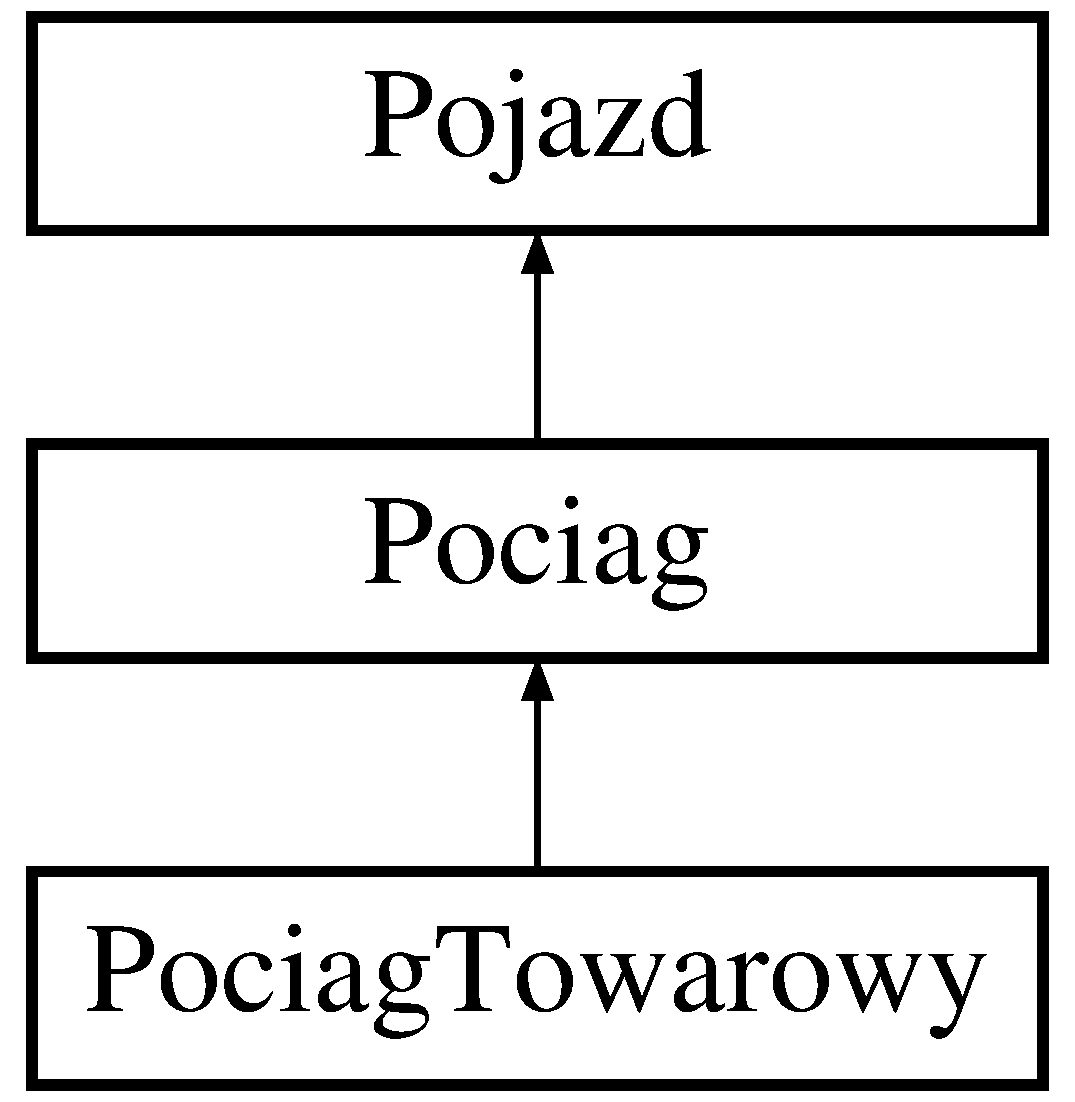
\includegraphics[height=3.000000cm]{class_pociag_towarowy}
\end{center}
\end{figure}
\subsection*{Public Member Functions}
\begin{DoxyCompactItemize}
\item 
\textbf{ Pociag\+Towarowy} ()
\begin{DoxyCompactList}\small\item\em Konstruktor domyślny. \end{DoxyCompactList}\item 
\textbf{ $\sim$\+Pociag\+Towarowy} ()
\begin{DoxyCompactList}\small\item\em Destruktor. \end{DoxyCompactList}\item 
void \textbf{ wyswietl\+Dane} ()
\begin{DoxyCompactList}\small\item\em Funkcja wirtualna wyświetlająca dane pociągu towarowego. \end{DoxyCompactList}\item 
void \textbf{ zmien\+Kolor} (string nowy\+\_\+kolor\+\_\+pociagu\+\_\+towarowego)
\item 
void \textbf{ dodaj\+Towar} (string nowy\+\_\+rodzaj\+\_\+towaru, int nowa\+\_\+waga\+\_\+towaru\+\_\+w\+\_\+tonach)
\item 
void \textbf{ zapisz} (\textbf{ Pociag\+Towarowy} \&pociag)
\item 
void \textbf{ odczytaj} (\textbf{ Pociag\+Towarowy} \&pociag)
\end{DoxyCompactItemize}
\subsection*{Friends}
\begin{DoxyCompactItemize}
\item 
ostream \& \textbf{ operator$<$$<$} (ostream \&s, \textbf{ Pociag\+Towarowy} \&p)
\begin{DoxyCompactList}\small\item\em Operator strumieniowy $<$$<$. \end{DoxyCompactList}\item 
istream \& \textbf{ operator$>$$>$} (istream \&s, \textbf{ Pociag\+Towarowy} \&p)
\begin{DoxyCompactList}\small\item\em Operator strumieniowy $>$$>$ \end{DoxyCompactList}\end{DoxyCompactItemize}
\subsection*{Additional Inherited Members}


\subsection{Detailed Description}
Klasa \doxyref{Pociag\+Towarowy}{p.}{class_pociag_towarowy}, pochodna klasy \doxyref{Pociag}{p.}{class_pociag}. 

\subsection{Constructor \& Destructor Documentation}
\mbox{\label{class_pociag_towarowy_ade86d8df7d23d1747d7f2a02893eaa25}} 
\index{Pociag\+Towarowy@{Pociag\+Towarowy}!Pociag\+Towarowy@{Pociag\+Towarowy}}
\index{Pociag\+Towarowy@{Pociag\+Towarowy}!Pociag\+Towarowy@{Pociag\+Towarowy}}
\subsubsection{Pociag\+Towarowy()}
{\footnotesize\ttfamily Pociag\+Towarowy\+::\+Pociag\+Towarowy (\begin{DoxyParamCaption}{ }\end{DoxyParamCaption})}



Konstruktor domyślny. 

\mbox{\label{class_pociag_towarowy_a18b830bad103982b34108498e6fb6e6c}} 
\index{Pociag\+Towarowy@{Pociag\+Towarowy}!````~Pociag\+Towarowy@{$\sim$\+Pociag\+Towarowy}}
\index{````~Pociag\+Towarowy@{$\sim$\+Pociag\+Towarowy}!Pociag\+Towarowy@{Pociag\+Towarowy}}
\subsubsection{$\sim$\+Pociag\+Towarowy()}
{\footnotesize\ttfamily Pociag\+Towarowy\+::$\sim$\+Pociag\+Towarowy (\begin{DoxyParamCaption}{ }\end{DoxyParamCaption})}



Destruktor. 



\subsection{Member Function Documentation}
\mbox{\label{class_pociag_towarowy_a945ec8897f6acbccf30b8c7d04dcafbb}} 
\index{Pociag\+Towarowy@{Pociag\+Towarowy}!dodaj\+Towar@{dodaj\+Towar}}
\index{dodaj\+Towar@{dodaj\+Towar}!Pociag\+Towarowy@{Pociag\+Towarowy}}
\subsubsection{dodaj\+Towar()}
{\footnotesize\ttfamily void Pociag\+Towarowy\+::dodaj\+Towar (\begin{DoxyParamCaption}\item[{string}]{nowy\+\_\+rodzaj\+\_\+towaru,  }\item[{int}]{nowa\+\_\+waga\+\_\+towaru\+\_\+w\+\_\+tonach }\end{DoxyParamCaption})}

Funckcja dodająca towar . Jako parametry podawany jest rodzaj towaru i jego waga 
\begin{DoxyParams}{Parameters}
{\em nowy\+\_\+rodzaj\+\_\+towaru} & określa rodzaj towaru \\
\hline
{\em nowa\+\_\+waga\+\_\+towaru\+\_\+w\+\_\+tonach} & określa wage towaru w tonach \\
\hline
\end{DoxyParams}
\begin{DoxyReturn}{Returns}
Funkcja nie zwraca żadnej wartości 
\end{DoxyReturn}
\mbox{\label{class_pociag_towarowy_a794490e9f983f873e8d075f35dc96325}} 
\index{Pociag\+Towarowy@{Pociag\+Towarowy}!odczytaj@{odczytaj}}
\index{odczytaj@{odczytaj}!Pociag\+Towarowy@{Pociag\+Towarowy}}
\subsubsection{odczytaj()}
{\footnotesize\ttfamily void Pociag\+Towarowy\+::odczytaj (\begin{DoxyParamCaption}\item[{\textbf{ Pociag\+Towarowy} \&}]{pociag }\end{DoxyParamCaption})}

Funkcja wczytująca pociąg towarowy z pliku Jako parametr przyjmuje obiekt pociąg towarowy i wczytuje do niego informacje z pliku 
\begin{DoxyParams}{Parameters}
{\em pociag} & określa pociag towarowy do którego wczytujemy dane \\
\hline
\end{DoxyParams}
\mbox{\label{class_pociag_towarowy_a5842dc6e39b23a6f6ca3c1f5edf36c6f}} 
\index{Pociag\+Towarowy@{Pociag\+Towarowy}!wyswietl\+Dane@{wyswietl\+Dane}}
\index{wyswietl\+Dane@{wyswietl\+Dane}!Pociag\+Towarowy@{Pociag\+Towarowy}}
\subsubsection{wyswietl\+Dane()}
{\footnotesize\ttfamily void Pociag\+Towarowy\+::wyswietl\+Dane (\begin{DoxyParamCaption}{ }\end{DoxyParamCaption})\hspace{0.3cm}{\ttfamily [virtual]}}



Funkcja wirtualna wyświetlająca dane pociągu towarowego. 



Implements \textbf{ Pojazd} \doxyref{}{p.}{class_pojazd_a945485210fbea0be179644bd68863304}.

\mbox{\label{class_pociag_towarowy_a30a1b2d5308f5cdafd07823bc07bccb4}} 
\index{Pociag\+Towarowy@{Pociag\+Towarowy}!zapisz@{zapisz}}
\index{zapisz@{zapisz}!Pociag\+Towarowy@{Pociag\+Towarowy}}
\subsubsection{zapisz()}
{\footnotesize\ttfamily void Pociag\+Towarowy\+::zapisz (\begin{DoxyParamCaption}\item[{\textbf{ Pociag\+Towarowy} \&}]{pociag }\end{DoxyParamCaption})}

Funkcja zapisująca pociąg towarowy do pliku Jako parametr przyjmuje obiekt pociąg towarowy i zapisuje informacje o nim do pliku 
\begin{DoxyParams}{Parameters}
{\em pociag} & określa pociag towarowy który zapisujemy \\
\hline
\end{DoxyParams}
\mbox{\label{class_pociag_towarowy_a25cee1a8b4b53a1e9b02f31672977e09}} 
\index{Pociag\+Towarowy@{Pociag\+Towarowy}!zmien\+Kolor@{zmien\+Kolor}}
\index{zmien\+Kolor@{zmien\+Kolor}!Pociag\+Towarowy@{Pociag\+Towarowy}}
\subsubsection{zmien\+Kolor()}
{\footnotesize\ttfamily void Pociag\+Towarowy\+::zmien\+Kolor (\begin{DoxyParamCaption}\item[{string}]{nowy\+\_\+kolor\+\_\+pociagu\+\_\+towarowego }\end{DoxyParamCaption})\hspace{0.3cm}{\ttfamily [virtual]}}

Funckcja wirtualna zmieniająca kolor pociągu towarowego. Jako parametr podawany jest nowy kolor pociągu towarowego /param nowy\+\_\+kolor określa kolor pociągu towarowego /return Funkcja nie zwraca żadnej wartości 

Implements \textbf{ Pojazd} \doxyref{}{p.}{class_pojazd_a29cab7cc8f5b4b3faed884f0d2849f4f}.



\subsection{Friends And Related Function Documentation}
\mbox{\label{class_pociag_towarowy_a46791b0f101793f7313aafa2eade03de}} 
\index{Pociag\+Towarowy@{Pociag\+Towarowy}!operator$<$$<$@{operator$<$$<$}}
\index{operator$<$$<$@{operator$<$$<$}!Pociag\+Towarowy@{Pociag\+Towarowy}}
\subsubsection{operator$<$$<$}
{\footnotesize\ttfamily ostream\& operator$<$$<$ (\begin{DoxyParamCaption}\item[{ostream \&}]{s,  }\item[{\textbf{ Pociag\+Towarowy} \&}]{p }\end{DoxyParamCaption})\hspace{0.3cm}{\ttfamily [friend]}}



Operator strumieniowy $<$$<$. 

\mbox{\label{class_pociag_towarowy_a4e728073e8406d3398d1b7c4afa2f0a2}} 
\index{Pociag\+Towarowy@{Pociag\+Towarowy}!operator$>$$>$@{operator$>$$>$}}
\index{operator$>$$>$@{operator$>$$>$}!Pociag\+Towarowy@{Pociag\+Towarowy}}
\subsubsection{operator$>$$>$}
{\footnotesize\ttfamily istream\& operator$>$$>$ (\begin{DoxyParamCaption}\item[{istream \&}]{s,  }\item[{\textbf{ Pociag\+Towarowy} \&}]{p }\end{DoxyParamCaption})\hspace{0.3cm}{\ttfamily [friend]}}



Operator strumieniowy $>$$>$ 



The documentation for this class was generated from the following files\+:\begin{DoxyCompactItemize}
\item 
\textbf{ Pociag towarowy.\+h}\item 
\textbf{ Pociag towarowy.\+cpp}\end{DoxyCompactItemize}

\section{Pojazd Class Reference}
\label{class_pojazd}\index{Pojazd@{Pojazd}}


Klasa abstrakcyjna.  




{\ttfamily \#include $<$Pojazd.\+h$>$}

Inheritance diagram for Pojazd\+:\begin{figure}[H]
\begin{center}
\leavevmode
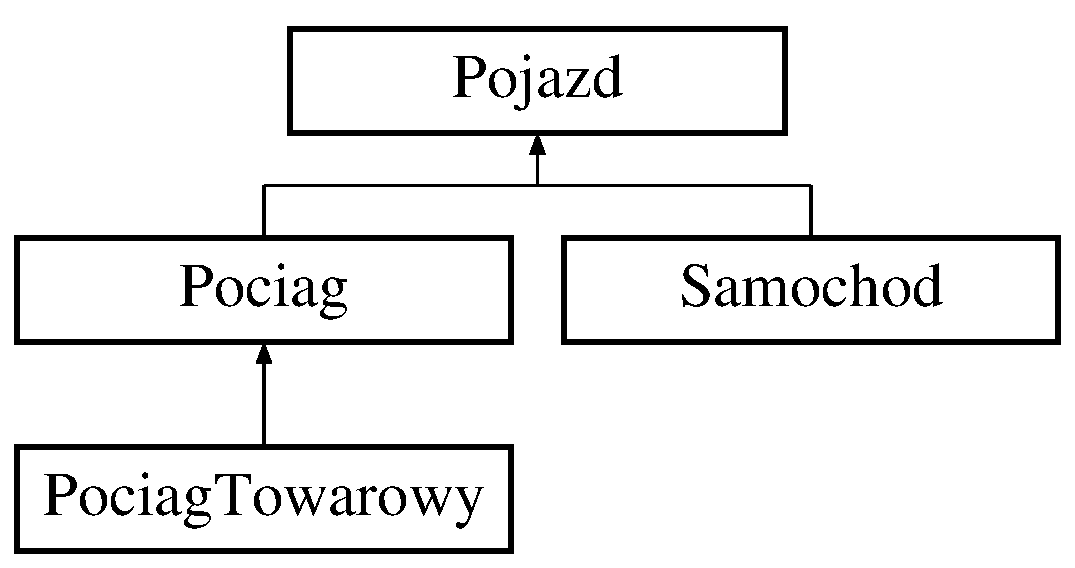
\includegraphics[height=3.000000cm]{class_pojazd}
\end{center}
\end{figure}
\subsection*{Public Member Functions}
\begin{DoxyCompactItemize}
\item 
\textbf{ Pojazd} ()
\begin{DoxyCompactList}\small\item\em Konstruktor domyślny. \end{DoxyCompactList}\item 
virtual \textbf{ $\sim$\+Pojazd} ()
\begin{DoxyCompactList}\small\item\em Destruktor wirtualny. \end{DoxyCompactList}\item 
virtual void \textbf{ wyswietl\+Dane} ()=0
\begin{DoxyCompactList}\small\item\em Procedura wirtualna. \end{DoxyCompactList}\item 
virtual void \textbf{ zmien\+Kolor} (string \textbf{ nowy\+\_\+kolor})=0
\begin{DoxyCompactList}\small\item\em Procedura wirtualna. \end{DoxyCompactList}\item 
virtual void \textbf{ zapisz} (\textbf{ Pojazd} \&pojazd)
\begin{DoxyCompactList}\small\item\em Procedura wirtualna. \end{DoxyCompactList}\item 
virtual void \textbf{ odczytaj} (\textbf{ Pojazd} \&pojazd)
\begin{DoxyCompactList}\small\item\em Procedura wirtualna. \end{DoxyCompactList}\end{DoxyCompactItemize}
\subsection*{Protected Attributes}
\begin{DoxyCompactItemize}
\item 
int \textbf{ rok\+\_\+produkcji}
\begin{DoxyCompactList}\small\item\em określa rok produkcji pojazdu \end{DoxyCompactList}\item 
string \textbf{ kolor}
\begin{DoxyCompactList}\small\item\em określa kolor pojazdu \end{DoxyCompactList}\end{DoxyCompactItemize}
\subsection*{Friends}
\begin{DoxyCompactItemize}
\item 
std\+::ostream \& \textbf{ operator$<$$<$} (std\+::ostream \&s, \textbf{ Pojazd} \&p)
\begin{DoxyCompactList}\small\item\em Operator strumieniowy $<$$<$. \end{DoxyCompactList}\item 
std\+::istream \& \textbf{ operator$>$$>$} (std\+::istream \&s, \textbf{ Pojazd} \&p)
\begin{DoxyCompactList}\small\item\em Operator strumieniowy $>$$>$ \end{DoxyCompactList}\end{DoxyCompactItemize}


\subsection{Detailed Description}
Klasa abstrakcyjna. 

\subsection{Constructor \& Destructor Documentation}
\mbox{\label{class_pojazd_adadab8f8cbb436d300d788314781a420}} 
\index{Pojazd@{Pojazd}!Pojazd@{Pojazd}}
\index{Pojazd@{Pojazd}!Pojazd@{Pojazd}}
\subsubsection{Pojazd()}
{\footnotesize\ttfamily Pojazd\+::\+Pojazd (\begin{DoxyParamCaption}{ }\end{DoxyParamCaption})}



Konstruktor domyślny. 

\mbox{\label{class_pojazd_a8fa527112445a2d598eff371f9f51039}} 
\index{Pojazd@{Pojazd}!````~Pojazd@{$\sim$\+Pojazd}}
\index{````~Pojazd@{$\sim$\+Pojazd}!Pojazd@{Pojazd}}
\subsubsection{$\sim$\+Pojazd()}
{\footnotesize\ttfamily Pojazd\+::$\sim$\+Pojazd (\begin{DoxyParamCaption}{ }\end{DoxyParamCaption})\hspace{0.3cm}{\ttfamily [virtual]}}



Destruktor wirtualny. 



\subsection{Member Function Documentation}
\mbox{\label{class_pojazd_ae527b4efc07951fc944e0c76f1db27ac}} 
\index{Pojazd@{Pojazd}!odczytaj@{odczytaj}}
\index{odczytaj@{odczytaj}!Pojazd@{Pojazd}}
\subsubsection{odczytaj()}
{\footnotesize\ttfamily void Pojazd\+::odczytaj (\begin{DoxyParamCaption}\item[{\textbf{ Pojazd} \&}]{pojazd }\end{DoxyParamCaption})\hspace{0.3cm}{\ttfamily [virtual]}}



Procedura wirtualna. 

\mbox{\label{class_pojazd_a945485210fbea0be179644bd68863304}} 
\index{Pojazd@{Pojazd}!wyswietl\+Dane@{wyswietl\+Dane}}
\index{wyswietl\+Dane@{wyswietl\+Dane}!Pojazd@{Pojazd}}
\subsubsection{wyswietl\+Dane()}
{\footnotesize\ttfamily virtual void Pojazd\+::wyswietl\+Dane (\begin{DoxyParamCaption}{ }\end{DoxyParamCaption})\hspace{0.3cm}{\ttfamily [pure virtual]}}



Procedura wirtualna. 



Implemented in \textbf{ Pociag} \doxyref{}{p.}{class_pociag_a1096a05d2981c1da0ac50870d37c1ffb}, \textbf{ Samochod} \doxyref{}{p.}{class_samochod_a34b47cf70e5e6ed83be62f3ad8d3cd63}, and \textbf{ Pociag\+Towarowy} \doxyref{}{p.}{class_pociag_towarowy_a5842dc6e39b23a6f6ca3c1f5edf36c6f}.

\mbox{\label{class_pojazd_af459a2afa32cbe2f54a74ec2f623c1fd}} 
\index{Pojazd@{Pojazd}!zapisz@{zapisz}}
\index{zapisz@{zapisz}!Pojazd@{Pojazd}}
\subsubsection{zapisz()}
{\footnotesize\ttfamily void Pojazd\+::zapisz (\begin{DoxyParamCaption}\item[{\textbf{ Pojazd} \&}]{pojazd }\end{DoxyParamCaption})\hspace{0.3cm}{\ttfamily [virtual]}}



Procedura wirtualna. 

\mbox{\label{class_pojazd_a29cab7cc8f5b4b3faed884f0d2849f4f}} 
\index{Pojazd@{Pojazd}!zmien\+Kolor@{zmien\+Kolor}}
\index{zmien\+Kolor@{zmien\+Kolor}!Pojazd@{Pojazd}}
\subsubsection{zmien\+Kolor()}
{\footnotesize\ttfamily virtual void Pojazd\+::zmien\+Kolor (\begin{DoxyParamCaption}\item[{string}]{nowy\+\_\+kolor }\end{DoxyParamCaption})\hspace{0.3cm}{\ttfamily [pure virtual]}}



Procedura wirtualna. 



Implemented in \textbf{ Pociag} \doxyref{}{p.}{class_pociag_a5645f7c8f4019124e63e41444b6893b4}, \textbf{ Samochod} \doxyref{}{p.}{class_samochod_ad06a48772ec0bfe426eecf0377a266bf}, and \textbf{ Pociag\+Towarowy} \doxyref{}{p.}{class_pociag_towarowy_a25cee1a8b4b53a1e9b02f31672977e09}.



\subsection{Friends And Related Function Documentation}
\mbox{\label{class_pojazd_a3c3d50c9fa2eb85fabaf027bbaf2ffda}} 
\index{Pojazd@{Pojazd}!operator$<$$<$@{operator$<$$<$}}
\index{operator$<$$<$@{operator$<$$<$}!Pojazd@{Pojazd}}
\subsubsection{operator$<$$<$}
{\footnotesize\ttfamily std\+::ostream\& operator$<$$<$ (\begin{DoxyParamCaption}\item[{std\+::ostream \&}]{s,  }\item[{\textbf{ Pojazd} \&}]{p }\end{DoxyParamCaption})\hspace{0.3cm}{\ttfamily [friend]}}



Operator strumieniowy $<$$<$. 

\mbox{\label{class_pojazd_aa0fa6911e723f94e1326ef19bcde5cff}} 
\index{Pojazd@{Pojazd}!operator$>$$>$@{operator$>$$>$}}
\index{operator$>$$>$@{operator$>$$>$}!Pojazd@{Pojazd}}
\subsubsection{operator$>$$>$}
{\footnotesize\ttfamily std\+::istream\& operator$>$$>$ (\begin{DoxyParamCaption}\item[{std\+::istream \&}]{s,  }\item[{\textbf{ Pojazd} \&}]{p }\end{DoxyParamCaption})\hspace{0.3cm}{\ttfamily [friend]}}



Operator strumieniowy $>$$>$ 



\subsection{Member Data Documentation}
\mbox{\label{class_pojazd_a5043f471a137e6dd705796d1293fcedf}} 
\index{Pojazd@{Pojazd}!kolor@{kolor}}
\index{kolor@{kolor}!Pojazd@{Pojazd}}
\subsubsection{kolor}
{\footnotesize\ttfamily string Pojazd\+::kolor\hspace{0.3cm}{\ttfamily [protected]}}



określa kolor pojazdu 

\mbox{\label{class_pojazd_a2bb8c2ae5639b420fe97b32c21f45d61}} 
\index{Pojazd@{Pojazd}!rok\+\_\+produkcji@{rok\+\_\+produkcji}}
\index{rok\+\_\+produkcji@{rok\+\_\+produkcji}!Pojazd@{Pojazd}}
\subsubsection{rok\+\_\+produkcji}
{\footnotesize\ttfamily int Pojazd\+::rok\+\_\+produkcji\hspace{0.3cm}{\ttfamily [protected]}}



określa rok produkcji pojazdu 



The documentation for this class was generated from the following files\+:\begin{DoxyCompactItemize}
\item 
\textbf{ Pojazd.\+h}\item 
\textbf{ Pojazd.\+cpp}\end{DoxyCompactItemize}

\section{Pracownik Class Reference}
\label{class_pracownik}\index{Pracownik@{Pracownik}}


Klasa \doxyref{Pracownik}{p.}{class_pracownik}, podklasa klasy \doxyref{Pociag}{p.}{class_pociag}.  




{\ttfamily \#include $<$pracownik.\+h$>$}

\subsection*{Public Member Functions}
\begin{DoxyCompactItemize}
\item 
\textbf{ Pracownik} ()
\begin{DoxyCompactList}\small\item\em Konstruktor domyślny. \end{DoxyCompactList}\item 
\textbf{ $\sim$\+Pracownik} ()
\begin{DoxyCompactList}\small\item\em Destruktor. \end{DoxyCompactList}\item 
void \textbf{ wypis\+Danych\+Pracownika} ()
\begin{DoxyCompactList}\small\item\em Funkcja wypisująca dane pracownika. \end{DoxyCompactList}\item 
void \textbf{ dodaj\+Dane\+Pracownika} (string nowy\+\_\+imie\+\_\+nazwisko, string nowy\+\_\+zawod, int nowy\+\_\+zarobki)
\item 
void \textbf{ zapisz} (\textbf{ Pracownik} \&pracownicy)
\item 
void \textbf{ wczytaj} (\textbf{ Pracownik} \&pracownicy)
\end{DoxyCompactItemize}
\subsection*{Friends}
\begin{DoxyCompactItemize}
\item 
ostream \& \textbf{ operator$<$$<$} (ostream \&s, \textbf{ Pracownik} \&p)
\begin{DoxyCompactList}\small\item\em Operator strumieniowy $<$$<$. \end{DoxyCompactList}\item 
istream \& \textbf{ operator$>$$>$} (istream \&s, \textbf{ Pracownik} \&p)
\begin{DoxyCompactList}\small\item\em Operator strumieniowy $>$$>$ \end{DoxyCompactList}\end{DoxyCompactItemize}


\subsection{Detailed Description}
Klasa \doxyref{Pracownik}{p.}{class_pracownik}, podklasa klasy \doxyref{Pociag}{p.}{class_pociag}. 

\subsection{Constructor \& Destructor Documentation}
\mbox{\label{class_pracownik_adae7e8f0ec1088ab80c4cbb3559cc628}} 
\index{Pracownik@{Pracownik}!Pracownik@{Pracownik}}
\index{Pracownik@{Pracownik}!Pracownik@{Pracownik}}
\subsubsection{Pracownik()}
{\footnotesize\ttfamily Pracownik\+::\+Pracownik (\begin{DoxyParamCaption}{ }\end{DoxyParamCaption})}



Konstruktor domyślny. 

\mbox{\label{class_pracownik_a2e8aa510eda960582b0c28d1fbd376d3}} 
\index{Pracownik@{Pracownik}!````~Pracownik@{$\sim$\+Pracownik}}
\index{````~Pracownik@{$\sim$\+Pracownik}!Pracownik@{Pracownik}}
\subsubsection{$\sim$\+Pracownik()}
{\footnotesize\ttfamily Pracownik\+::$\sim$\+Pracownik (\begin{DoxyParamCaption}{ }\end{DoxyParamCaption})}



Destruktor. 



\subsection{Member Function Documentation}
\mbox{\label{class_pracownik_a20664a92d253cd014aee538805a147c1}} 
\index{Pracownik@{Pracownik}!dodaj\+Dane\+Pracownika@{dodaj\+Dane\+Pracownika}}
\index{dodaj\+Dane\+Pracownika@{dodaj\+Dane\+Pracownika}!Pracownik@{Pracownik}}
\subsubsection{dodaj\+Dane\+Pracownika()}
{\footnotesize\ttfamily void Pracownik\+::dodaj\+Dane\+Pracownika (\begin{DoxyParamCaption}\item[{string}]{nowy\+\_\+imie\+\_\+nazwisko,  }\item[{string}]{nowy\+\_\+zawod,  }\item[{int}]{nowy\+\_\+zarobki }\end{DoxyParamCaption})}

Procedura dodająca dane pracownika. Jako parametry przyjmuje imie i nazwisko pracownika, zawód i zarobki 
\begin{DoxyParams}{Parameters}
{\em nowy\+\_\+imie\+\_\+nazwisko} & określa imię i nazwisko pracownika \\
\hline
{\em nowy\+\_\+zawod} & określa zawód pracownika \\
\hline
{\em nowy\+\_\+zarobki} & określa zarobki pracownika \\
\hline
\end{DoxyParams}
\begin{DoxyReturn}{Returns}
Funkcja nie zwraca żadnej wartości 
\end{DoxyReturn}
\mbox{\label{class_pracownik_a41aa35381636e38a51d3dc0c095c521b}} 
\index{Pracownik@{Pracownik}!wczytaj@{wczytaj}}
\index{wczytaj@{wczytaj}!Pracownik@{Pracownik}}
\subsubsection{wczytaj()}
{\footnotesize\ttfamily void Pracownik\+::wczytaj (\begin{DoxyParamCaption}\item[{\textbf{ Pracownik} \&}]{pracownicy }\end{DoxyParamCaption})}

Funkcja wczytujące dane z pliku pracownikom Jako parametr przyjmuje kontener zawierający pracowników i wczytuje im dane z pliku 
\begin{DoxyParams}{Parameters}
{\em pracownicy} & określa pracowników którym wczytujemy dane \\
\hline
\end{DoxyParams}
\mbox{\label{class_pracownik_aea06aff33ba401709b83be10303e87c2}} 
\index{Pracownik@{Pracownik}!wypis\+Danych\+Pracownika@{wypis\+Danych\+Pracownika}}
\index{wypis\+Danych\+Pracownika@{wypis\+Danych\+Pracownika}!Pracownik@{Pracownik}}
\subsubsection{wypis\+Danych\+Pracownika()}
{\footnotesize\ttfamily void Pracownik\+::wypis\+Danych\+Pracownika (\begin{DoxyParamCaption}{ }\end{DoxyParamCaption})}



Funkcja wypisująca dane pracownika. 

\mbox{\label{class_pracownik_ad5a74efa1cadcf8dc6a2730141833a43}} 
\index{Pracownik@{Pracownik}!zapisz@{zapisz}}
\index{zapisz@{zapisz}!Pracownik@{Pracownik}}
\subsubsection{zapisz()}
{\footnotesize\ttfamily void Pracownik\+::zapisz (\begin{DoxyParamCaption}\item[{\textbf{ Pracownik} \&}]{pracownicy }\end{DoxyParamCaption})}

Funkcja zapisująca dane pracownikó do pliku Jako parametr przyjmuje kontener zawierający pracowników i zapisuje informacje o nich do pliku 
\begin{DoxyParams}{Parameters}
{\em pracownicy} & określa pracowników których zapisujemy \\
\hline
\end{DoxyParams}


\subsection{Friends And Related Function Documentation}
\mbox{\label{class_pracownik_a178bdb8fdeb19bc53a50422983104895}} 
\index{Pracownik@{Pracownik}!operator$<$$<$@{operator$<$$<$}}
\index{operator$<$$<$@{operator$<$$<$}!Pracownik@{Pracownik}}
\subsubsection{operator$<$$<$}
{\footnotesize\ttfamily ostream\& operator$<$$<$ (\begin{DoxyParamCaption}\item[{ostream \&}]{s,  }\item[{\textbf{ Pracownik} \&}]{p }\end{DoxyParamCaption})\hspace{0.3cm}{\ttfamily [friend]}}



Operator strumieniowy $<$$<$. 

\mbox{\label{class_pracownik_a514d9af5b092da25ac1cf108d6cb9069}} 
\index{Pracownik@{Pracownik}!operator$>$$>$@{operator$>$$>$}}
\index{operator$>$$>$@{operator$>$$>$}!Pracownik@{Pracownik}}
\subsubsection{operator$>$$>$}
{\footnotesize\ttfamily istream\& operator$>$$>$ (\begin{DoxyParamCaption}\item[{istream \&}]{s,  }\item[{\textbf{ Pracownik} \&}]{p }\end{DoxyParamCaption})\hspace{0.3cm}{\ttfamily [friend]}}



Operator strumieniowy $>$$>$ 



The documentation for this class was generated from the following files\+:\begin{DoxyCompactItemize}
\item 
\textbf{ pracownik.\+h}\item 
\textbf{ pracownik.\+cpp}\end{DoxyCompactItemize}

\section{Samochod Class Reference}
\label{class_samochod}\index{Samochod@{Samochod}}


Klasa \doxyref{Samochod}{p.}{class_samochod}, pochodna klasy \doxyref{Pojazd}{p.}{class_pojazd}.  




{\ttfamily \#include $<$Samochód.\+h$>$}

Inheritance diagram for Samochod\+:\begin{figure}[H]
\begin{center}
\leavevmode
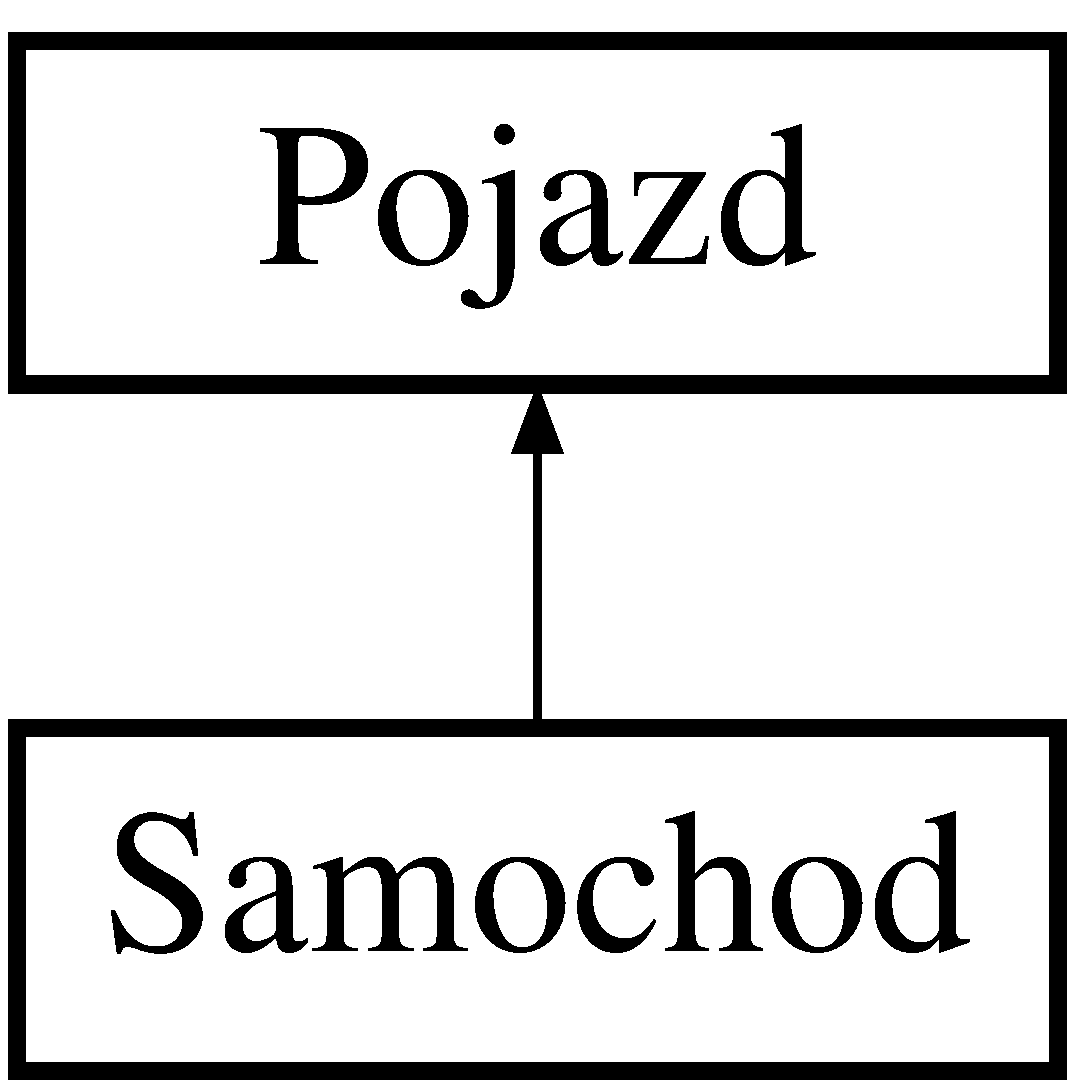
\includegraphics[height=2.000000cm]{class_samochod}
\end{center}
\end{figure}
\subsection*{Public Member Functions}
\begin{DoxyCompactItemize}
\item 
\textbf{ Samochod} ()
\begin{DoxyCompactList}\small\item\em Konstruktor domyślny. \end{DoxyCompactList}\item 
\textbf{ $\sim$\+Samochod} ()
\begin{DoxyCompactList}\small\item\em Destruktor. \end{DoxyCompactList}\item 
\textbf{ Samochod} (string n\+\_\+marka, string n\+\_\+typ\+\_\+samochodu, int n\+\_\+rok\+\_\+produkcji, string n\+\_\+kolor)
\item 
void \textbf{ wyswietl\+Dane} ()
\begin{DoxyCompactList}\small\item\em Funkcja wirtualna wyświetlająca dane samochodu. \end{DoxyCompactList}\item 
void \textbf{ zmien\+Kolor} (string nowy\+\_\+kolor\+\_\+samochodu)
\begin{DoxyCompactList}\small\item\em Funkcja wirtuaolna zmieniająca kolor samochodu. \end{DoxyCompactList}\item 
void \textbf{ zapisz} (\textbf{ Samochod} \&samochod)
\item 
void \textbf{ wczytaj} (\textbf{ Samochod} \&samochod)
\end{DoxyCompactItemize}
\subsection*{Friends}
\begin{DoxyCompactItemize}
\item 
ostream \& \textbf{ operator$<$$<$} (ostream \&s, \textbf{ Samochod} \&c)
\begin{DoxyCompactList}\small\item\em Operator strumieniowy $<$$<$. \end{DoxyCompactList}\item 
istream \& \textbf{ operator$>$$>$} (istream \&s, \textbf{ Samochod} \&c)
\begin{DoxyCompactList}\small\item\em Operator strumieniowy $>$$>$ \end{DoxyCompactList}\end{DoxyCompactItemize}
\subsection*{Additional Inherited Members}


\subsection{Detailed Description}
Klasa \doxyref{Samochod}{p.}{class_samochod}, pochodna klasy \doxyref{Pojazd}{p.}{class_pojazd}. 

\subsection{Constructor \& Destructor Documentation}
\mbox{\label{class_samochod_a56ae27a3e568333f010604249d463c96}} 
\index{Samochod@{Samochod}!Samochod@{Samochod}}
\index{Samochod@{Samochod}!Samochod@{Samochod}}
\subsubsection{Samochod()\hspace{0.1cm}{\footnotesize\ttfamily [1/2]}}
{\footnotesize\ttfamily Samochod\+::\+Samochod (\begin{DoxyParamCaption}{ }\end{DoxyParamCaption})}



Konstruktor domyślny. 

\mbox{\label{class_samochod_a5995c359256c60addb4b362c2797b37c}} 
\index{Samochod@{Samochod}!````~Samochod@{$\sim$\+Samochod}}
\index{````~Samochod@{$\sim$\+Samochod}!Samochod@{Samochod}}
\subsubsection{$\sim$\+Samochod()}
{\footnotesize\ttfamily Samochod\+::$\sim$\+Samochod (\begin{DoxyParamCaption}{ }\end{DoxyParamCaption})}



Destruktor. 

\mbox{\label{class_samochod_aff378f2f87df7f8d8562dddb37cb5cf4}} 
\index{Samochod@{Samochod}!Samochod@{Samochod}}
\index{Samochod@{Samochod}!Samochod@{Samochod}}
\subsubsection{Samochod()\hspace{0.1cm}{\footnotesize\ttfamily [2/2]}}
{\footnotesize\ttfamily Samochod\+::\+Samochod (\begin{DoxyParamCaption}\item[{string}]{n\+\_\+marka,  }\item[{string}]{n\+\_\+typ\+\_\+samochodu,  }\item[{int}]{n\+\_\+rok\+\_\+produkcji,  }\item[{string}]{n\+\_\+kolor }\end{DoxyParamCaption})}

Konstruktor Przyjmuje jako parametry marke, typ samochodu, rok produkcji i kolor 
\begin{DoxyParams}{Parameters}
{\em n\+\_\+marka} & określa markę samochodu \\
\hline
{\em n\+\_\+typ\+\_\+samochodu} & określa typ samochodu \\
\hline
{\em n\+\_\+rok\+\_\+produkcji} & określa rok produkcji samochodu \\
\hline
{\em n\+\_\+kolor} & określa kolor samochodu \\
\hline
\end{DoxyParams}
\begin{DoxyReturn}{Returns}
Konstruktor nie zwraca żadnej wartości 
\end{DoxyReturn}


\subsection{Member Function Documentation}
\mbox{\label{class_samochod_a78ba738ef76bf9d1344a19dcee5c38bc}} 
\index{Samochod@{Samochod}!wczytaj@{wczytaj}}
\index{wczytaj@{wczytaj}!Samochod@{Samochod}}
\subsubsection{wczytaj()}
{\footnotesize\ttfamily void Samochod\+::wczytaj (\begin{DoxyParamCaption}\item[{\textbf{ Samochod} \&}]{samochod }\end{DoxyParamCaption})}

Funkcja wczytująca obiekt z pliku Jako parametr przyjmuje obiekt samochod i wczytuje do niego informacje z pliku 
\begin{DoxyParams}{Parameters}
{\em pociag} & określa samochód do którego wczytujemy dane \\
\hline
\end{DoxyParams}
\mbox{\label{class_samochod_a34b47cf70e5e6ed83be62f3ad8d3cd63}} 
\index{Samochod@{Samochod}!wyswietl\+Dane@{wyswietl\+Dane}}
\index{wyswietl\+Dane@{wyswietl\+Dane}!Samochod@{Samochod}}
\subsubsection{wyswietl\+Dane()}
{\footnotesize\ttfamily void Samochod\+::wyswietl\+Dane (\begin{DoxyParamCaption}{ }\end{DoxyParamCaption})\hspace{0.3cm}{\ttfamily [virtual]}}



Funkcja wirtualna wyświetlająca dane samochodu. 



Implements \textbf{ Pojazd} \doxyref{}{p.}{class_pojazd_a945485210fbea0be179644bd68863304}.

\mbox{\label{class_samochod_a73499649dc66eb93763a979cbe31f421}} 
\index{Samochod@{Samochod}!zapisz@{zapisz}}
\index{zapisz@{zapisz}!Samochod@{Samochod}}
\subsubsection{zapisz()}
{\footnotesize\ttfamily void Samochod\+::zapisz (\begin{DoxyParamCaption}\item[{\textbf{ Samochod} \&}]{samochod }\end{DoxyParamCaption})}

Funkcja zapisująca samochód do pliku Jako parametr przyjmuje obiekt samochod i zapisuje informacje o nim do pliku 
\begin{DoxyParams}{Parameters}
{\em samochod} & określa pociag którego dane zapisujemy \\
\hline
\end{DoxyParams}
\mbox{\label{class_samochod_ad06a48772ec0bfe426eecf0377a266bf}} 
\index{Samochod@{Samochod}!zmien\+Kolor@{zmien\+Kolor}}
\index{zmien\+Kolor@{zmien\+Kolor}!Samochod@{Samochod}}
\subsubsection{zmien\+Kolor()}
{\footnotesize\ttfamily void Samochod\+::zmien\+Kolor (\begin{DoxyParamCaption}\item[{string}]{nowy\+\_\+kolor\+\_\+samochodu }\end{DoxyParamCaption})\hspace{0.3cm}{\ttfamily [virtual]}}



Funkcja wirtuaolna zmieniająca kolor samochodu. 



Implements \textbf{ Pojazd} \doxyref{}{p.}{class_pojazd_a29cab7cc8f5b4b3faed884f0d2849f4f}.



\subsection{Friends And Related Function Documentation}
\mbox{\label{class_samochod_a6c050739ef12b1dda9845e2d107c61ca}} 
\index{Samochod@{Samochod}!operator$<$$<$@{operator$<$$<$}}
\index{operator$<$$<$@{operator$<$$<$}!Samochod@{Samochod}}
\subsubsection{operator$<$$<$}
{\footnotesize\ttfamily ostream\& operator$<$$<$ (\begin{DoxyParamCaption}\item[{ostream \&}]{s,  }\item[{\textbf{ Samochod} \&}]{c }\end{DoxyParamCaption})\hspace{0.3cm}{\ttfamily [friend]}}



Operator strumieniowy $<$$<$. 

\mbox{\label{class_samochod_a6bf080449778fa75622f3e10731f414d}} 
\index{Samochod@{Samochod}!operator$>$$>$@{operator$>$$>$}}
\index{operator$>$$>$@{operator$>$$>$}!Samochod@{Samochod}}
\subsubsection{operator$>$$>$}
{\footnotesize\ttfamily istream\& operator$>$$>$ (\begin{DoxyParamCaption}\item[{istream \&}]{s,  }\item[{\textbf{ Samochod} \&}]{c }\end{DoxyParamCaption})\hspace{0.3cm}{\ttfamily [friend]}}



Operator strumieniowy $>$$>$ 



The documentation for this class was generated from the following files\+:\begin{DoxyCompactItemize}
\item 
\textbf{ Samochód.\+h}\item 
\textbf{ Samochód.\+cpp}\end{DoxyCompactItemize}

\section{Trasa Class Reference}
\label{class_trasa}\index{Trasa@{Trasa}}


Klasa \doxyref{Trasa}{p.}{class_trasa}, podklasa klasy \doxyref{Pociag}{p.}{class_pociag}.  




{\ttfamily \#include $<$trasa.\+h$>$}

\subsection*{Public Member Functions}
\begin{DoxyCompactItemize}
\item 
\textbf{ Trasa} ()
\begin{DoxyCompactList}\small\item\em Konstruktor domyślny. \end{DoxyCompactList}\item 
\textbf{ $\sim$\+Trasa} ()
\begin{DoxyCompactList}\small\item\em Destruktor. \end{DoxyCompactList}\item 
void \textbf{ wypis\+Danych\+Trasy} ()
\begin{DoxyCompactList}\small\item\em Funkcja wypisująca informacje o trasie. \end{DoxyCompactList}\item 
void \textbf{ dodaj\+Dane\+Trasy} (string poczatek\+\_\+t, string koniec\+\_\+t, int czas\+\_\+przejazdu, int dlugosc\+\_\+t)
\item 
void \textbf{ dodaj\+Opoznienie} (int opoznienie)
\item 
void \textbf{ zapisz} (\textbf{ Trasa} \&trasa)
\item 
void \textbf{ wczytaj} (\textbf{ Trasa} \&trasa)
\item 
bool \textbf{ operator$>$} (const \textbf{ Trasa} \&t)
\begin{DoxyCompactList}\small\item\em Operator $>$ \end{DoxyCompactList}\item 
bool \textbf{ operator$<$} (const \textbf{ Trasa} \&t)
\begin{DoxyCompactList}\small\item\em Operator $<$. \end{DoxyCompactList}\item 
\textbf{ Trasa} \textbf{ operator+} (const \textbf{ Trasa} \&t)
\begin{DoxyCompactList}\small\item\em Operator +. \end{DoxyCompactList}\end{DoxyCompactItemize}
\subsection*{Friends}
\begin{DoxyCompactItemize}
\item 
ostream \& \textbf{ operator$<$$<$} (ostream \&s, \textbf{ Trasa} \&t)
\begin{DoxyCompactList}\small\item\em Operator strumieniowy $<$$<$. \end{DoxyCompactList}\item 
istream \& \textbf{ operator$>$$>$} (istream \&s, \textbf{ Trasa} \&t)
\begin{DoxyCompactList}\small\item\em Operator strumieniowy $>$$>$ \end{DoxyCompactList}\end{DoxyCompactItemize}


\subsection{Detailed Description}
Klasa \doxyref{Trasa}{p.}{class_trasa}, podklasa klasy \doxyref{Pociag}{p.}{class_pociag}. 

\subsection{Constructor \& Destructor Documentation}
\mbox{\label{class_trasa_a5f18e484a5335c0f5f7d030ca984717f}} 
\index{Trasa@{Trasa}!Trasa@{Trasa}}
\index{Trasa@{Trasa}!Trasa@{Trasa}}
\subsubsection{Trasa()}
{\footnotesize\ttfamily Trasa\+::\+Trasa (\begin{DoxyParamCaption}{ }\end{DoxyParamCaption})}



Konstruktor domyślny. 

\mbox{\label{class_trasa_a42ba4ee49a8937f527d5fd5a9971434c}} 
\index{Trasa@{Trasa}!````~Trasa@{$\sim$\+Trasa}}
\index{````~Trasa@{$\sim$\+Trasa}!Trasa@{Trasa}}
\subsubsection{$\sim$\+Trasa()}
{\footnotesize\ttfamily Trasa\+::$\sim$\+Trasa (\begin{DoxyParamCaption}{ }\end{DoxyParamCaption})}



Destruktor. 



\subsection{Member Function Documentation}
\mbox{\label{class_trasa_a3b0aa4c583d8fd0902ad88f645249c02}} 
\index{Trasa@{Trasa}!dodaj\+Dane\+Trasy@{dodaj\+Dane\+Trasy}}
\index{dodaj\+Dane\+Trasy@{dodaj\+Dane\+Trasy}!Trasa@{Trasa}}
\subsubsection{dodaj\+Dane\+Trasy()}
{\footnotesize\ttfamily void Trasa\+::dodaj\+Dane\+Trasy (\begin{DoxyParamCaption}\item[{string}]{poczatek\+\_\+t,  }\item[{string}]{koniec\+\_\+t,  }\item[{int}]{czas\+\_\+przejazdu,  }\item[{int}]{dlugosc\+\_\+t }\end{DoxyParamCaption})}

Funkcja dodająca dane o trasie Jako parametry przyjmuje początek i koniec trasy, czas przejazdu i długość trasy 
\begin{DoxyParams}{Parameters}
{\em poczatek\+\_\+t} & określa początek trasy pociągu \\
\hline
{\em koniec\+\_\+t} & określa koniec trasy pociągu \\
\hline
{\em czas\+\_\+przejazdu} & określa czas przejazdu pociągu \\
\hline
{\em dlugosc\+\_\+t} & określa długość trasy w kilometrach \\
\hline
\end{DoxyParams}
\begin{DoxyReturn}{Returns}
Funkcja nie zwraca żadnej wartości 
\end{DoxyReturn}
\mbox{\label{class_trasa_a6e7959bcac1db9c4116f990676a12e65}} 
\index{Trasa@{Trasa}!dodaj\+Opoznienie@{dodaj\+Opoznienie}}
\index{dodaj\+Opoznienie@{dodaj\+Opoznienie}!Trasa@{Trasa}}
\subsubsection{dodaj\+Opoznienie()}
{\footnotesize\ttfamily void Trasa\+::dodaj\+Opoznienie (\begin{DoxyParamCaption}\item[{int}]{opoznienie }\end{DoxyParamCaption})}

Funkcja dodająca opóźnienie na trasie Jako parametr przyjmuje długość opóźnienia w minutach 
\begin{DoxyParams}{Parameters}
{\em opoznienie} & określa długość opóźniena pociągu w minutach \\
\hline
\end{DoxyParams}
\begin{DoxyReturn}{Returns}
Funkcja nie zwraca żadnej wartości 
\end{DoxyReturn}
\mbox{\label{class_trasa_a562c8e38ff046b57d6ea5e60ec598e51}} 
\index{Trasa@{Trasa}!operator+@{operator+}}
\index{operator+@{operator+}!Trasa@{Trasa}}
\subsubsection{operator+()}
{\footnotesize\ttfamily \textbf{ Trasa} Trasa\+::operator+ (\begin{DoxyParamCaption}\item[{const \textbf{ Trasa} \&}]{t }\end{DoxyParamCaption})}



Operator +. 

\mbox{\label{class_trasa_a23b4e087865aef23f45c21c21ef5ccdd}} 
\index{Trasa@{Trasa}!operator$<$@{operator$<$}}
\index{operator$<$@{operator$<$}!Trasa@{Trasa}}
\subsubsection{operator$<$()}
{\footnotesize\ttfamily bool Trasa\+::operator$<$ (\begin{DoxyParamCaption}\item[{const \textbf{ Trasa} \&}]{t }\end{DoxyParamCaption})}



Operator $<$. 

\mbox{\label{class_trasa_a942b3732d4814ad0764f964e0282d216}} 
\index{Trasa@{Trasa}!operator$>$@{operator$>$}}
\index{operator$>$@{operator$>$}!Trasa@{Trasa}}
\subsubsection{operator$>$()}
{\footnotesize\ttfamily bool Trasa\+::operator$>$ (\begin{DoxyParamCaption}\item[{const \textbf{ Trasa} \&}]{t }\end{DoxyParamCaption})}



Operator $>$ 

\mbox{\label{class_trasa_a2283be5d0139fd35a9cd0e40eb6ede1b}} 
\index{Trasa@{Trasa}!wczytaj@{wczytaj}}
\index{wczytaj@{wczytaj}!Trasa@{Trasa}}
\subsubsection{wczytaj()}
{\footnotesize\ttfamily void Trasa\+::wczytaj (\begin{DoxyParamCaption}\item[{\textbf{ Trasa} \&}]{trasa }\end{DoxyParamCaption})}

Funkcja wczytująca obiekt z pliku Jako parametr przyjmuje obiekt trasa i wczytuje do niego informacje z pliku 
\begin{DoxyParams}{Parameters}
{\em trasa} & określa pociag do którego wczytujemy dane \\
\hline
\end{DoxyParams}
\mbox{\label{class_trasa_a3e3d0447d1bff7a8798f52d28dc414d8}} 
\index{Trasa@{Trasa}!wypis\+Danych\+Trasy@{wypis\+Danych\+Trasy}}
\index{wypis\+Danych\+Trasy@{wypis\+Danych\+Trasy}!Trasa@{Trasa}}
\subsubsection{wypis\+Danych\+Trasy()}
{\footnotesize\ttfamily void Trasa\+::wypis\+Danych\+Trasy (\begin{DoxyParamCaption}{ }\end{DoxyParamCaption})}



Funkcja wypisująca informacje o trasie. 

\mbox{\label{class_trasa_a81f175a914fd02eaf6019696a79d7785}} 
\index{Trasa@{Trasa}!zapisz@{zapisz}}
\index{zapisz@{zapisz}!Trasa@{Trasa}}
\subsubsection{zapisz()}
{\footnotesize\ttfamily void Trasa\+::zapisz (\begin{DoxyParamCaption}\item[{\textbf{ Trasa} \&}]{trasa }\end{DoxyParamCaption})}

Funkcja zapisująca trase do pliku Jako parametr przyjmuje obiekt trase i zapisuje informacje o niej do pliku 
\begin{DoxyParams}{Parameters}
{\em trasa} & określa trase, której dane zapisujemy \\
\hline
\end{DoxyParams}


\subsection{Friends And Related Function Documentation}
\mbox{\label{class_trasa_a546eedc44ac2ff4fcf2d361a8f08d9b0}} 
\index{Trasa@{Trasa}!operator$<$$<$@{operator$<$$<$}}
\index{operator$<$$<$@{operator$<$$<$}!Trasa@{Trasa}}
\subsubsection{operator$<$$<$}
{\footnotesize\ttfamily ostream\& operator$<$$<$ (\begin{DoxyParamCaption}\item[{ostream \&}]{s,  }\item[{\textbf{ Trasa} \&}]{t }\end{DoxyParamCaption})\hspace{0.3cm}{\ttfamily [friend]}}



Operator strumieniowy $<$$<$. 

\mbox{\label{class_trasa_ad5f6762bbed1b1cf1bf3c1c647830346}} 
\index{Trasa@{Trasa}!operator$>$$>$@{operator$>$$>$}}
\index{operator$>$$>$@{operator$>$$>$}!Trasa@{Trasa}}
\subsubsection{operator$>$$>$}
{\footnotesize\ttfamily istream\& operator$>$$>$ (\begin{DoxyParamCaption}\item[{istream \&}]{s,  }\item[{\textbf{ Trasa} \&}]{t }\end{DoxyParamCaption})\hspace{0.3cm}{\ttfamily [friend]}}



Operator strumieniowy $>$$>$ 



The documentation for this class was generated from the following files\+:\begin{DoxyCompactItemize}
\item 
\textbf{ trasa.\+h}\item 
\textbf{ trasa.\+cpp}\end{DoxyCompactItemize}

\section{Wagony Class Reference}
\label{class_wagony}\index{Wagony@{Wagony}}


Klasa \doxyref{Wagony}{p.}{class_wagony}, podklasa klasy \doxyref{Pociag}{p.}{class_pociag}.  




{\ttfamily \#include $<$wagony.\+h$>$}

\subsection*{Public Member Functions}
\begin{DoxyCompactItemize}
\item 
\textbf{ Wagony} ()
\begin{DoxyCompactList}\small\item\em Konstruktor domyślny. \end{DoxyCompactList}\item 
\textbf{ $\sim$\+Wagony} ()
\begin{DoxyCompactList}\small\item\em Destruktor. \end{DoxyCompactList}\item 
void \textbf{ wypis\+Danych\+Wagonow} ()
\begin{DoxyCompactList}\small\item\em Funkcja wypisująca dane o wagonach. \end{DoxyCompactList}\item 
void \textbf{ dodaj\+Dane\+Wagonow} (int liczba\+\_\+w)
\item 
void \textbf{ dodaj\+Wagony} (int ile\+\_\+wagonow)
\item 
void \textbf{ zapisz} (\textbf{ Wagony} \&wagony)
\item 
void \textbf{ wczytaj} (\textbf{ Wagony} \&wagony)
\item 
bool \textbf{ operator==} (const \textbf{ Wagony} \&w)
\begin{DoxyCompactList}\small\item\em Operator ==. \end{DoxyCompactList}\item 
bool \textbf{ operator$>$} (const \textbf{ Wagony} \&w)
\begin{DoxyCompactList}\small\item\em Operator $>$ \end{DoxyCompactList}\item 
bool \textbf{ operator$<$} (const \textbf{ Wagony} \&w)
\begin{DoxyCompactList}\small\item\em Operator $<$. \end{DoxyCompactList}\item 
\textbf{ Wagony} \textbf{ operator+} (const \textbf{ Wagony} \&w)
\begin{DoxyCompactList}\small\item\em Operator +. \end{DoxyCompactList}\end{DoxyCompactItemize}
\subsection*{Friends}
\begin{DoxyCompactItemize}
\item 
ostream \& \textbf{ operator$<$$<$} (ostream \&s, \textbf{ Wagony} \&w)
\begin{DoxyCompactList}\small\item\em Operator stumieniowy $<$$<$. \end{DoxyCompactList}\item 
istream \& \textbf{ operator$>$$>$} (istream \&s, \textbf{ Wagony} \&w)
\begin{DoxyCompactList}\small\item\em Operator strumieniowy $>$$>$ \end{DoxyCompactList}\end{DoxyCompactItemize}


\subsection{Detailed Description}
Klasa \doxyref{Wagony}{p.}{class_wagony}, podklasa klasy \doxyref{Pociag}{p.}{class_pociag}. 

\subsection{Constructor \& Destructor Documentation}
\mbox{\label{class_wagony_a6a2b51627882c3dfcc7ede62bc328264}} 
\index{Wagony@{Wagony}!Wagony@{Wagony}}
\index{Wagony@{Wagony}!Wagony@{Wagony}}
\subsubsection{Wagony()}
{\footnotesize\ttfamily Wagony\+::\+Wagony (\begin{DoxyParamCaption}{ }\end{DoxyParamCaption})}



Konstruktor domyślny. 

\mbox{\label{class_wagony_a25c4689606486f86836f16a4a96e9a93}} 
\index{Wagony@{Wagony}!````~Wagony@{$\sim$\+Wagony}}
\index{````~Wagony@{$\sim$\+Wagony}!Wagony@{Wagony}}
\subsubsection{$\sim$\+Wagony()}
{\footnotesize\ttfamily Wagony\+::$\sim$\+Wagony (\begin{DoxyParamCaption}{ }\end{DoxyParamCaption})}



Destruktor. 



\subsection{Member Function Documentation}
\mbox{\label{class_wagony_afbc932d950bda3f21248494c4d7396dc}} 
\index{Wagony@{Wagony}!dodaj\+Dane\+Wagonow@{dodaj\+Dane\+Wagonow}}
\index{dodaj\+Dane\+Wagonow@{dodaj\+Dane\+Wagonow}!Wagony@{Wagony}}
\subsubsection{dodaj\+Dane\+Wagonow()}
{\footnotesize\ttfamily void Wagony\+::dodaj\+Dane\+Wagonow (\begin{DoxyParamCaption}\item[{int}]{liczba\+\_\+w }\end{DoxyParamCaption})}

Funkcja dodająca dane o wagonach Przyjmuje jako parametr liczbę wagonów 
\begin{DoxyParams}{Parameters}
{\em liczba\+\_\+w} & określa liczbę wagonów \\
\hline
\end{DoxyParams}
\begin{DoxyReturn}{Returns}
Funkcja nie zwraca żadnej wartości 
\end{DoxyReturn}
\mbox{\label{class_wagony_adb948fbe49fd7936c74f210502936437}} 
\index{Wagony@{Wagony}!dodaj\+Wagony@{dodaj\+Wagony}}
\index{dodaj\+Wagony@{dodaj\+Wagony}!Wagony@{Wagony}}
\subsubsection{dodaj\+Wagony()}
{\footnotesize\ttfamily void Wagony\+::dodaj\+Wagony (\begin{DoxyParamCaption}\item[{int}]{ile\+\_\+wagonow }\end{DoxyParamCaption})}

Funkcja zmieniająca liczbe wagonów Jako parametr przyjmuje nowy liczbe wagonów 
\begin{DoxyParams}{Parameters}
{\em ile\+\_\+wagonow} & określa liczbe wagonów \\
\hline
\end{DoxyParams}
\begin{DoxyReturn}{Returns}
Funkcja nie zwraca żadnej wartości 
\end{DoxyReturn}
\mbox{\label{class_wagony_a928b5138130f51c7d98bb85fbed9113b}} 
\index{Wagony@{Wagony}!operator+@{operator+}}
\index{operator+@{operator+}!Wagony@{Wagony}}
\subsubsection{operator+()}
{\footnotesize\ttfamily \textbf{ Wagony} Wagony\+::operator+ (\begin{DoxyParamCaption}\item[{const \textbf{ Wagony} \&}]{w }\end{DoxyParamCaption})}



Operator +. 

\mbox{\label{class_wagony_a357eae15892590c097f8d775cea3f3bf}} 
\index{Wagony@{Wagony}!operator$<$@{operator$<$}}
\index{operator$<$@{operator$<$}!Wagony@{Wagony}}
\subsubsection{operator$<$()}
{\footnotesize\ttfamily bool Wagony\+::operator$<$ (\begin{DoxyParamCaption}\item[{const \textbf{ Wagony} \&}]{w }\end{DoxyParamCaption})}



Operator $<$. 

\mbox{\label{class_wagony_a760a73d7cd21736a9a68c7c841880193}} 
\index{Wagony@{Wagony}!operator==@{operator==}}
\index{operator==@{operator==}!Wagony@{Wagony}}
\subsubsection{operator==()}
{\footnotesize\ttfamily bool Wagony\+::operator== (\begin{DoxyParamCaption}\item[{const \textbf{ Wagony} \&}]{w }\end{DoxyParamCaption})}



Operator ==. 

\mbox{\label{class_wagony_a5da51cfa75005428038d0e09d7f2d47f}} 
\index{Wagony@{Wagony}!operator$>$@{operator$>$}}
\index{operator$>$@{operator$>$}!Wagony@{Wagony}}
\subsubsection{operator$>$()}
{\footnotesize\ttfamily bool Wagony\+::operator$>$ (\begin{DoxyParamCaption}\item[{const \textbf{ Wagony} \&}]{w }\end{DoxyParamCaption})}



Operator $>$ 

\mbox{\label{class_wagony_a30dff1d362283dfe86061f69c09d4a33}} 
\index{Wagony@{Wagony}!wczytaj@{wczytaj}}
\index{wczytaj@{wczytaj}!Wagony@{Wagony}}
\subsubsection{wczytaj()}
{\footnotesize\ttfamily void Wagony\+::wczytaj (\begin{DoxyParamCaption}\item[{\textbf{ Wagony} \&}]{wagony }\end{DoxyParamCaption})}

Funkcja wczytująca obiekt z pliku Jako parametr przyjmuje obiekt wagony i wczytuje do niego informacje z pliku 
\begin{DoxyParams}{Parameters}
{\em wagony} & określa trase do którego wczytujemy dane \\
\hline
\end{DoxyParams}
\mbox{\label{class_wagony_af703b28fadd78b088ae63b0cd56d6be7}} 
\index{Wagony@{Wagony}!wypis\+Danych\+Wagonow@{wypis\+Danych\+Wagonow}}
\index{wypis\+Danych\+Wagonow@{wypis\+Danych\+Wagonow}!Wagony@{Wagony}}
\subsubsection{wypis\+Danych\+Wagonow()}
{\footnotesize\ttfamily void Wagony\+::wypis\+Danych\+Wagonow (\begin{DoxyParamCaption}{ }\end{DoxyParamCaption})}



Funkcja wypisująca dane o wagonach. 

\mbox{\label{class_wagony_a9cf2b865118b388a0aab4dc28261ffa2}} 
\index{Wagony@{Wagony}!zapisz@{zapisz}}
\index{zapisz@{zapisz}!Wagony@{Wagony}}
\subsubsection{zapisz()}
{\footnotesize\ttfamily void Wagony\+::zapisz (\begin{DoxyParamCaption}\item[{\textbf{ Wagony} \&}]{wagony }\end{DoxyParamCaption})}

Funkcja wczytująca obiekt z pliku Jako parametr przyjmuje obiekt wagony i wczytuje do niego informacje z pliku 
\begin{DoxyParams}{Parameters}
{\em wagony} & określa pociag do którego wczytujemy dane \\
\hline
\end{DoxyParams}


\subsection{Friends And Related Function Documentation}
\mbox{\label{class_wagony_a1829f200bc2533d2cc98ec9e17e2174e}} 
\index{Wagony@{Wagony}!operator$<$$<$@{operator$<$$<$}}
\index{operator$<$$<$@{operator$<$$<$}!Wagony@{Wagony}}
\subsubsection{operator$<$$<$}
{\footnotesize\ttfamily ostream\& operator$<$$<$ (\begin{DoxyParamCaption}\item[{ostream \&}]{s,  }\item[{\textbf{ Wagony} \&}]{w }\end{DoxyParamCaption})\hspace{0.3cm}{\ttfamily [friend]}}



Operator stumieniowy $<$$<$. 

\mbox{\label{class_wagony_a55e031de3cc9ab883ab9356fda851f11}} 
\index{Wagony@{Wagony}!operator$>$$>$@{operator$>$$>$}}
\index{operator$>$$>$@{operator$>$$>$}!Wagony@{Wagony}}
\subsubsection{operator$>$$>$}
{\footnotesize\ttfamily istream\& operator$>$$>$ (\begin{DoxyParamCaption}\item[{istream \&}]{s,  }\item[{\textbf{ Wagony} \&}]{w }\end{DoxyParamCaption})\hspace{0.3cm}{\ttfamily [friend]}}



Operator strumieniowy $>$$>$ 



The documentation for this class was generated from the following files\+:\begin{DoxyCompactItemize}
\item 
\textbf{ wagony.\+h}\item 
\textbf{ wagony.\+cpp}\end{DoxyCompactItemize}

\chapter{File Documentation}
\section{Pociag towarowy.\+cpp File Reference}
\label{_pociag_01towarowy_8cpp}\index{Pociag towarowy.\+cpp@{Pociag towarowy.\+cpp}}
{\ttfamily \#include \char`\"{}Pociag towarowy.\+h\char`\"{}}\newline
{\ttfamily \#include $<$iostream$>$}\newline
{\ttfamily \#include $<$fstream$>$}\newline
\subsection*{Functions}
\begin{DoxyCompactItemize}
\item 
ostream \& \textbf{ operator$<$$<$} (ostream \&s, \textbf{ Pociag\+Towarowy} \&p)
\item 
istream \& \textbf{ operator$>$$>$} (istream \&s, \textbf{ Pociag\+Towarowy} \&p)
\end{DoxyCompactItemize}
\subsection*{Variables}
\begin{DoxyCompactItemize}
\item 
string \textbf{ nazwa\+\_\+pliku\+\_\+po\+\_\+towa} = \char`\"{}pociag towarowy.\+txt\char`\"{}
\end{DoxyCompactItemize}


\subsection{Function Documentation}
\mbox{\label{_pociag_01towarowy_8cpp_a46791b0f101793f7313aafa2eade03de}} 
\index{Pociag towarowy.\+cpp@{Pociag towarowy.\+cpp}!operator$<$$<$@{operator$<$$<$}}
\index{operator$<$$<$@{operator$<$$<$}!Pociag towarowy.\+cpp@{Pociag towarowy.\+cpp}}
\subsubsection{operator$<$$<$()}
{\footnotesize\ttfamily ostream\& operator$<$$<$ (\begin{DoxyParamCaption}\item[{ostream \&}]{s,  }\item[{\textbf{ Pociag\+Towarowy} \&}]{p }\end{DoxyParamCaption})}

\mbox{\label{_pociag_01towarowy_8cpp_a4e728073e8406d3398d1b7c4afa2f0a2}} 
\index{Pociag towarowy.\+cpp@{Pociag towarowy.\+cpp}!operator$>$$>$@{operator$>$$>$}}
\index{operator$>$$>$@{operator$>$$>$}!Pociag towarowy.\+cpp@{Pociag towarowy.\+cpp}}
\subsubsection{operator$>$$>$()}
{\footnotesize\ttfamily istream\& operator$>$$>$ (\begin{DoxyParamCaption}\item[{istream \&}]{s,  }\item[{\textbf{ Pociag\+Towarowy} \&}]{p }\end{DoxyParamCaption})}



\subsection{Variable Documentation}
\mbox{\label{_pociag_01towarowy_8cpp_aca8140573b982a119b54e71d26b15f7a}} 
\index{Pociag towarowy.\+cpp@{Pociag towarowy.\+cpp}!nazwa\+\_\+pliku\+\_\+po\+\_\+towa@{nazwa\+\_\+pliku\+\_\+po\+\_\+towa}}
\index{nazwa\+\_\+pliku\+\_\+po\+\_\+towa@{nazwa\+\_\+pliku\+\_\+po\+\_\+towa}!Pociag towarowy.\+cpp@{Pociag towarowy.\+cpp}}
\subsubsection{nazwa\+\_\+pliku\+\_\+po\+\_\+towa}
{\footnotesize\ttfamily string nazwa\+\_\+pliku\+\_\+po\+\_\+towa = \char`\"{}pociag towarowy.\+txt\char`\"{}}


\section{Pociag towarowy.\+h File Reference}
\label{_pociag_01towarowy_8h}\index{Pociag towarowy.\+h@{Pociag towarowy.\+h}}
{\ttfamily \#include \char`\"{}pociag.\+h\char`\"{}}\newline
\subsection*{Classes}
\begin{DoxyCompactItemize}
\item 
class \textbf{ Pociag\+Towarowy}
\begin{DoxyCompactList}\small\item\em Klasa \doxyref{Pociag\+Towarowy}{p.}{class_pociag_towarowy}, pochodna klasy \doxyref{Pociag}{p.}{class_pociag}. \end{DoxyCompactList}\end{DoxyCompactItemize}

\section{pociag.\+cpp File Reference}
\label{pociag_8cpp}\index{pociag.\+cpp@{pociag.\+cpp}}
{\ttfamily \#include $<$iostream$>$}\newline
{\ttfamily \#include $<$fstream$>$}\newline
{\ttfamily \#include $<$string$>$}\newline
{\ttfamily \#include $<$cmath$>$}\newline
{\ttfamily \#include \char`\"{}pociag.\+h\char`\"{}}\newline
\subsection*{Functions}
\begin{DoxyCompactItemize}
\item 
ostream \& \textbf{ operator$<$$<$} (ostream \&s, \textbf{ Pociag} \&p)
\item 
istream \& \textbf{ operator$>$$>$} (istream \&s, \textbf{ Pociag} \&p)
\end{DoxyCompactItemize}
\subsection*{Variables}
\begin{DoxyCompactItemize}
\item 
string \textbf{ nazwa\+\_\+pliku\+\_\+po} = \char`\"{}pociag.\+txt\char`\"{}
\end{DoxyCompactItemize}


\subsection{Function Documentation}
\mbox{\label{pociag_8cpp_aa69694c17cdb3e184cc54938668f705c}} 
\index{pociag.\+cpp@{pociag.\+cpp}!operator$<$$<$@{operator$<$$<$}}
\index{operator$<$$<$@{operator$<$$<$}!pociag.\+cpp@{pociag.\+cpp}}
\subsubsection{operator$<$$<$()}
{\footnotesize\ttfamily ostream\& operator$<$$<$ (\begin{DoxyParamCaption}\item[{ostream \&}]{s,  }\item[{\textbf{ Pociag} \&}]{p }\end{DoxyParamCaption})}

\mbox{\label{pociag_8cpp_a00926731077d7f0d7c1a81c50bee727d}} 
\index{pociag.\+cpp@{pociag.\+cpp}!operator$>$$>$@{operator$>$$>$}}
\index{operator$>$$>$@{operator$>$$>$}!pociag.\+cpp@{pociag.\+cpp}}
\subsubsection{operator$>$$>$()}
{\footnotesize\ttfamily istream\& operator$>$$>$ (\begin{DoxyParamCaption}\item[{istream \&}]{s,  }\item[{\textbf{ Pociag} \&}]{p }\end{DoxyParamCaption})}



\subsection{Variable Documentation}
\mbox{\label{pociag_8cpp_a5311644a6939f63f9bd0b8c1a7e3809b}} 
\index{pociag.\+cpp@{pociag.\+cpp}!nazwa\+\_\+pliku\+\_\+po@{nazwa\+\_\+pliku\+\_\+po}}
\index{nazwa\+\_\+pliku\+\_\+po@{nazwa\+\_\+pliku\+\_\+po}!pociag.\+cpp@{pociag.\+cpp}}
\subsubsection{nazwa\+\_\+pliku\+\_\+po}
{\footnotesize\ttfamily string nazwa\+\_\+pliku\+\_\+po = \char`\"{}pociag.\+txt\char`\"{}}


\section{pociag.\+h File Reference}
\label{pociag_8h}\index{pociag.\+h@{pociag.\+h}}
{\ttfamily \#include $<$string$>$}\newline
{\ttfamily \#include \char`\"{}pracownik.\+h\char`\"{}}\newline
{\ttfamily \#include \char`\"{}wagony.\+h\char`\"{}}\newline
{\ttfamily \#include \char`\"{}trasa.\+h\char`\"{}}\newline
{\ttfamily \#include \char`\"{}Pojazd.\+h\char`\"{}}\newline
{\ttfamily \#include \char`\"{}vector\char`\"{}}\newline
\subsection*{Classes}
\begin{DoxyCompactItemize}
\item 
class \textbf{ Pociag}
\begin{DoxyCompactList}\small\item\em Klasa Pociąg, pochodna klasy \doxyref{Pojazd}{p.}{class_pojazd}. \end{DoxyCompactList}\end{DoxyCompactItemize}

\section{Pojazd.\+cpp File Reference}
\label{_pojazd_8cpp}\index{Pojazd.\+cpp@{Pojazd.\+cpp}}
{\ttfamily \#include \char`\"{}Pojazd.\+h\char`\"{}}\newline
{\ttfamily \#include $<$iostream$>$}\newline
{\ttfamily \#include $<$fstream$>$}\newline
\subsection*{Functions}
\begin{DoxyCompactItemize}
\item 
std\+::ostream \& \textbf{ operator$<$$<$} (std\+::ostream \&s, \textbf{ Pojazd} \&p)
\item 
std\+::istream \& \textbf{ operator$>$$>$} (std\+::istream \&s, \textbf{ Pojazd} \&p)
\end{DoxyCompactItemize}
\subsection*{Variables}
\begin{DoxyCompactItemize}
\item 
string \textbf{ nazwa\+\_\+pliku\+\_\+poj} = \char`\"{}pojazd.\+txt\char`\"{}
\end{DoxyCompactItemize}


\subsection{Function Documentation}
\mbox{\label{_pojazd_8cpp_a3c3d50c9fa2eb85fabaf027bbaf2ffda}} 
\index{Pojazd.\+cpp@{Pojazd.\+cpp}!operator$<$$<$@{operator$<$$<$}}
\index{operator$<$$<$@{operator$<$$<$}!Pojazd.\+cpp@{Pojazd.\+cpp}}
\subsubsection{operator$<$$<$()}
{\footnotesize\ttfamily std\+::ostream\& operator$<$$<$ (\begin{DoxyParamCaption}\item[{std\+::ostream \&}]{s,  }\item[{\textbf{ Pojazd} \&}]{p }\end{DoxyParamCaption})}

\mbox{\label{_pojazd_8cpp_aa0fa6911e723f94e1326ef19bcde5cff}} 
\index{Pojazd.\+cpp@{Pojazd.\+cpp}!operator$>$$>$@{operator$>$$>$}}
\index{operator$>$$>$@{operator$>$$>$}!Pojazd.\+cpp@{Pojazd.\+cpp}}
\subsubsection{operator$>$$>$()}
{\footnotesize\ttfamily std\+::istream\& operator$>$$>$ (\begin{DoxyParamCaption}\item[{std\+::istream \&}]{s,  }\item[{\textbf{ Pojazd} \&}]{p }\end{DoxyParamCaption})}



\subsection{Variable Documentation}
\mbox{\label{_pojazd_8cpp_a2c1e9002ea68196e590270f9cbc05302}} 
\index{Pojazd.\+cpp@{Pojazd.\+cpp}!nazwa\+\_\+pliku\+\_\+poj@{nazwa\+\_\+pliku\+\_\+poj}}
\index{nazwa\+\_\+pliku\+\_\+poj@{nazwa\+\_\+pliku\+\_\+poj}!Pojazd.\+cpp@{Pojazd.\+cpp}}
\subsubsection{nazwa\+\_\+pliku\+\_\+poj}
{\footnotesize\ttfamily string nazwa\+\_\+pliku\+\_\+poj = \char`\"{}pojazd.\+txt\char`\"{}}


\section{Pojazd.\+h File Reference}
\label{_pojazd_8h}\index{Pojazd.\+h@{Pojazd.\+h}}
{\ttfamily \#include $<$string$>$}\newline
\subsection*{Classes}
\begin{DoxyCompactItemize}
\item 
class \textbf{ Pojazd}
\begin{DoxyCompactList}\small\item\em Klasa abstrakcyjna. \end{DoxyCompactList}\end{DoxyCompactItemize}

\section{pracownik.\+cpp File Reference}
\label{pracownik_8cpp}\index{pracownik.\+cpp@{pracownik.\+cpp}}
{\ttfamily \#include $<$iostream$>$}\newline
{\ttfamily \#include $<$fstream$>$}\newline
{\ttfamily \#include $<$string$>$}\newline
{\ttfamily \#include \char`\"{}pracownik.\+h\char`\"{}}\newline
\subsection*{Functions}
\begin{DoxyCompactItemize}
\item 
ostream \& \textbf{ operator$<$$<$} (ostream \&s, \textbf{ Pracownik} \&p)
\item 
istream \& \textbf{ operator$>$$>$} (istream \&s, \textbf{ Pracownik} \&p)
\end{DoxyCompactItemize}
\subsection*{Variables}
\begin{DoxyCompactItemize}
\item 
string \textbf{ nazwa\+\_\+pliku\+\_\+pra} = \char`\"{}pracownicy.\+txt\char`\"{}
\end{DoxyCompactItemize}


\subsection{Function Documentation}
\mbox{\label{pracownik_8cpp_a178bdb8fdeb19bc53a50422983104895}} 
\index{pracownik.\+cpp@{pracownik.\+cpp}!operator$<$$<$@{operator$<$$<$}}
\index{operator$<$$<$@{operator$<$$<$}!pracownik.\+cpp@{pracownik.\+cpp}}
\subsubsection{operator$<$$<$()}
{\footnotesize\ttfamily ostream\& operator$<$$<$ (\begin{DoxyParamCaption}\item[{ostream \&}]{s,  }\item[{\textbf{ Pracownik} \&}]{p }\end{DoxyParamCaption})}

\mbox{\label{pracownik_8cpp_a514d9af5b092da25ac1cf108d6cb9069}} 
\index{pracownik.\+cpp@{pracownik.\+cpp}!operator$>$$>$@{operator$>$$>$}}
\index{operator$>$$>$@{operator$>$$>$}!pracownik.\+cpp@{pracownik.\+cpp}}
\subsubsection{operator$>$$>$()}
{\footnotesize\ttfamily istream\& operator$>$$>$ (\begin{DoxyParamCaption}\item[{istream \&}]{s,  }\item[{\textbf{ Pracownik} \&}]{p }\end{DoxyParamCaption})}



\subsection{Variable Documentation}
\mbox{\label{pracownik_8cpp_ad819bf244f9d183b1fbc03a880d6169d}} 
\index{pracownik.\+cpp@{pracownik.\+cpp}!nazwa\+\_\+pliku\+\_\+pra@{nazwa\+\_\+pliku\+\_\+pra}}
\index{nazwa\+\_\+pliku\+\_\+pra@{nazwa\+\_\+pliku\+\_\+pra}!pracownik.\+cpp@{pracownik.\+cpp}}
\subsubsection{nazwa\+\_\+pliku\+\_\+pra}
{\footnotesize\ttfamily string nazwa\+\_\+pliku\+\_\+pra = \char`\"{}pracownicy.\+txt\char`\"{}}


\section{pracownik.\+h File Reference}
\label{pracownik_8h}\index{pracownik.\+h@{pracownik.\+h}}
{\ttfamily \#include $<$string$>$}\newline
\subsection*{Classes}
\begin{DoxyCompactItemize}
\item 
class \textbf{ Pracownik}
\begin{DoxyCompactList}\small\item\em Klasa \doxyref{Pracownik}{p.}{class_pracownik}, podklasa klasy \doxyref{Pociag}{p.}{class_pociag}. \end{DoxyCompactList}\end{DoxyCompactItemize}

\section{P\+R\+O\+J\+E\+K\+T.\+cpp File Reference}
\label{_p_r_o_j_e_k_t_8cpp}\index{P\+R\+O\+J\+E\+K\+T.\+cpp@{P\+R\+O\+J\+E\+K\+T.\+cpp}}
{\ttfamily \#include $<$string$>$}\newline
{\ttfamily \#include $<$iostream$>$}\newline
{\ttfamily \#include $<$fstream$>$}\newline
{\ttfamily \#include \char`\"{}trasa.\+h\char`\"{}}\newline
{\ttfamily \#include \char`\"{}wagony.\+h\char`\"{}}\newline
{\ttfamily \#include \char`\"{}pracownik.\+h\char`\"{}}\newline
{\ttfamily \#include \char`\"{}pociag.\+h\char`\"{}}\newline
{\ttfamily \#include \char`\"{}Pojazd.\+h\char`\"{}}\newline
{\ttfamily \#include \char`\"{}Pociag towarowy.\+h\char`\"{}}\newline
{\ttfamily \#include \char`\"{}Samochód.\+h\char`\"{}}\newline
\subsection*{Functions}
\begin{DoxyCompactItemize}
\item 
void \textbf{ test1} ()
\item 
int \textbf{ main} ()
\end{DoxyCompactItemize}
\subsection*{Variables}
\begin{DoxyCompactItemize}
\item 
string \textbf{ nowy\+\_\+kolor}
\item 
int \textbf{ opcja}
\item 
int \textbf{ obiekt}
\end{DoxyCompactItemize}


\subsection{Function Documentation}
\mbox{\label{_p_r_o_j_e_k_t_8cpp_ae66f6b31b5ad750f1fe042a706a4e3d4}} 
\index{P\+R\+O\+J\+E\+K\+T.\+cpp@{P\+R\+O\+J\+E\+K\+T.\+cpp}!main@{main}}
\index{main@{main}!P\+R\+O\+J\+E\+K\+T.\+cpp@{P\+R\+O\+J\+E\+K\+T.\+cpp}}
\subsubsection{main()}
{\footnotesize\ttfamily int main (\begin{DoxyParamCaption}{ }\end{DoxyParamCaption})}

\mbox{\label{_p_r_o_j_e_k_t_8cpp_a1440a7779ac56f47a3f355ce4a8c7da0}} 
\index{P\+R\+O\+J\+E\+K\+T.\+cpp@{P\+R\+O\+J\+E\+K\+T.\+cpp}!test1@{test1}}
\index{test1@{test1}!P\+R\+O\+J\+E\+K\+T.\+cpp@{P\+R\+O\+J\+E\+K\+T.\+cpp}}
\subsubsection{test1()}
{\footnotesize\ttfamily void test1 (\begin{DoxyParamCaption}{ }\end{DoxyParamCaption})}



\subsection{Variable Documentation}
\mbox{\label{_p_r_o_j_e_k_t_8cpp_aa42089d1169edfa73d76e296dbecf70c}} 
\index{P\+R\+O\+J\+E\+K\+T.\+cpp@{P\+R\+O\+J\+E\+K\+T.\+cpp}!nowy\+\_\+kolor@{nowy\+\_\+kolor}}
\index{nowy\+\_\+kolor@{nowy\+\_\+kolor}!P\+R\+O\+J\+E\+K\+T.\+cpp@{P\+R\+O\+J\+E\+K\+T.\+cpp}}
\subsubsection{nowy\+\_\+kolor}
{\footnotesize\ttfamily string nowy\+\_\+kolor}

\mbox{\label{_p_r_o_j_e_k_t_8cpp_ac06bfea83890bfc9fab70041705947be}} 
\index{P\+R\+O\+J\+E\+K\+T.\+cpp@{P\+R\+O\+J\+E\+K\+T.\+cpp}!obiekt@{obiekt}}
\index{obiekt@{obiekt}!P\+R\+O\+J\+E\+K\+T.\+cpp@{P\+R\+O\+J\+E\+K\+T.\+cpp}}
\subsubsection{obiekt}
{\footnotesize\ttfamily int obiekt}

\mbox{\label{_p_r_o_j_e_k_t_8cpp_adaeb9433eaa673c6d8c4793b5bfd9ec3}} 
\index{P\+R\+O\+J\+E\+K\+T.\+cpp@{P\+R\+O\+J\+E\+K\+T.\+cpp}!opcja@{opcja}}
\index{opcja@{opcja}!P\+R\+O\+J\+E\+K\+T.\+cpp@{P\+R\+O\+J\+E\+K\+T.\+cpp}}
\subsubsection{opcja}
{\footnotesize\ttfamily int opcja}


\section{Samochód.\+cpp File Reference}
\label{_samoch_xC3_xB3d_8cpp}\index{Samochód.\+cpp@{Samochód.\+cpp}}
{\ttfamily \#include \char`\"{}Samochód.\+h\char`\"{}}\newline
{\ttfamily \#include $<$fstream$>$}\newline
\subsection*{Functions}
\begin{DoxyCompactItemize}
\item 
ostream \& \textbf{ operator$<$$<$} (ostream \&s, \textbf{ Samochod} \&c)
\item 
istream \& \textbf{ operator$>$$>$} (istream \&s, \textbf{ Samochod} \&c)
\end{DoxyCompactItemize}
\subsection*{Variables}
\begin{DoxyCompactItemize}
\item 
string \textbf{ nazwa\+\_\+pliku\+\_\+sa} = \char`\"{}samochod.\+txt\char`\"{}
\end{DoxyCompactItemize}


\subsection{Function Documentation}
\mbox{\label{_samoch_xC3_xB3d_8cpp_a6c050739ef12b1dda9845e2d107c61ca}} 
\index{Samochód.\+cpp@{Samochód.\+cpp}!operator$<$$<$@{operator$<$$<$}}
\index{operator$<$$<$@{operator$<$$<$}!Samochód.\+cpp@{Samochód.\+cpp}}
\subsubsection{operator$<$$<$()}
{\footnotesize\ttfamily ostream\& operator$<$$<$ (\begin{DoxyParamCaption}\item[{ostream \&}]{s,  }\item[{\textbf{ Samochod} \&}]{c }\end{DoxyParamCaption})}

\mbox{\label{_samoch_xC3_xB3d_8cpp_a6bf080449778fa75622f3e10731f414d}} 
\index{Samochód.\+cpp@{Samochód.\+cpp}!operator$>$$>$@{operator$>$$>$}}
\index{operator$>$$>$@{operator$>$$>$}!Samochód.\+cpp@{Samochód.\+cpp}}
\subsubsection{operator$>$$>$()}
{\footnotesize\ttfamily istream\& operator$>$$>$ (\begin{DoxyParamCaption}\item[{istream \&}]{s,  }\item[{\textbf{ Samochod} \&}]{c }\end{DoxyParamCaption})}



\subsection{Variable Documentation}
\mbox{\label{_samoch_xC3_xB3d_8cpp_ad00380e35acedd3fbdbec3054f5ee17c}} 
\index{Samochód.\+cpp@{Samochód.\+cpp}!nazwa\+\_\+pliku\+\_\+sa@{nazwa\+\_\+pliku\+\_\+sa}}
\index{nazwa\+\_\+pliku\+\_\+sa@{nazwa\+\_\+pliku\+\_\+sa}!Samochód.\+cpp@{Samochód.\+cpp}}
\subsubsection{nazwa\+\_\+pliku\+\_\+sa}
{\footnotesize\ttfamily string nazwa\+\_\+pliku\+\_\+sa = \char`\"{}samochod.\+txt\char`\"{}}


\section{Samochód.\+h File Reference}
\label{_samoch_xC3_xB3d_8h}\index{Samochód.\+h@{Samochód.\+h}}
{\ttfamily \#include \char`\"{}Pojazd.\+h\char`\"{}}\newline
{\ttfamily \#include $<$iostream$>$}\newline
\subsection*{Classes}
\begin{DoxyCompactItemize}
\item 
class \textbf{ Samochod}
\begin{DoxyCompactList}\small\item\em Klasa \doxyref{Samochod}{p.}{class_samochod}, pochodna klasy \doxyref{Pojazd}{p.}{class_pojazd}. \end{DoxyCompactList}\end{DoxyCompactItemize}

\section{stdafx.\+cpp File Reference}
\label{stdafx_8cpp}\index{stdafx.\+cpp@{stdafx.\+cpp}}
{\ttfamily \#include \char`\"{}stdafx.\+h\char`\"{}}\newline

\section{stdafx.\+h File Reference}
\label{stdafx_8h}\index{stdafx.\+h@{stdafx.\+h}}
{\ttfamily \#include \char`\"{}targetver.\+h\char`\"{}}\newline
{\ttfamily \#include $<$stdio.\+h$>$}\newline
{\ttfamily \#include $<$tchar.\+h$>$}\newline

\section{targetver.\+h File Reference}
\label{targetver_8h}\index{targetver.\+h@{targetver.\+h}}
{\ttfamily \#include $<$S\+D\+K\+D\+D\+K\+Ver.\+h$>$}\newline

\section{trasa.\+cpp File Reference}
\label{trasa_8cpp}\index{trasa.\+cpp@{trasa.\+cpp}}
{\ttfamily \#include $<$iostream$>$}\newline
{\ttfamily \#include $<$fstream$>$}\newline
{\ttfamily \#include $<$string$>$}\newline
{\ttfamily \#include \char`\"{}trasa.\+h\char`\"{}}\newline
\subsection*{Functions}
\begin{DoxyCompactItemize}
\item 
ostream \& \textbf{ operator$<$$<$} (ostream \&s, \textbf{ Trasa} \&t)
\item 
istream \& \textbf{ operator$>$$>$} (istream \&s, \textbf{ Trasa} \&t)
\end{DoxyCompactItemize}
\subsection*{Variables}
\begin{DoxyCompactItemize}
\item 
string \textbf{ nazwa\+\_\+pliku\+\_\+t} = \char`\"{}trasa.\+txt\char`\"{}
\end{DoxyCompactItemize}


\subsection{Function Documentation}
\mbox{\label{trasa_8cpp_a546eedc44ac2ff4fcf2d361a8f08d9b0}} 
\index{trasa.\+cpp@{trasa.\+cpp}!operator$<$$<$@{operator$<$$<$}}
\index{operator$<$$<$@{operator$<$$<$}!trasa.\+cpp@{trasa.\+cpp}}
\subsubsection{operator$<$$<$()}
{\footnotesize\ttfamily ostream\& operator$<$$<$ (\begin{DoxyParamCaption}\item[{ostream \&}]{s,  }\item[{\textbf{ Trasa} \&}]{t }\end{DoxyParamCaption})}

\mbox{\label{trasa_8cpp_ad5f6762bbed1b1cf1bf3c1c647830346}} 
\index{trasa.\+cpp@{trasa.\+cpp}!operator$>$$>$@{operator$>$$>$}}
\index{operator$>$$>$@{operator$>$$>$}!trasa.\+cpp@{trasa.\+cpp}}
\subsubsection{operator$>$$>$()}
{\footnotesize\ttfamily istream\& operator$>$$>$ (\begin{DoxyParamCaption}\item[{istream \&}]{s,  }\item[{\textbf{ Trasa} \&}]{t }\end{DoxyParamCaption})}



\subsection{Variable Documentation}
\mbox{\label{trasa_8cpp_a071ca74a9d8c791ed69b52f0393d5487}} 
\index{trasa.\+cpp@{trasa.\+cpp}!nazwa\+\_\+pliku\+\_\+t@{nazwa\+\_\+pliku\+\_\+t}}
\index{nazwa\+\_\+pliku\+\_\+t@{nazwa\+\_\+pliku\+\_\+t}!trasa.\+cpp@{trasa.\+cpp}}
\subsubsection{nazwa\+\_\+pliku\+\_\+t}
{\footnotesize\ttfamily string nazwa\+\_\+pliku\+\_\+t = \char`\"{}trasa.\+txt\char`\"{}}


\section{trasa.\+h File Reference}
\label{trasa_8h}\index{trasa.\+h@{trasa.\+h}}
{\ttfamily \#include $<$string$>$}\newline
\subsection*{Classes}
\begin{DoxyCompactItemize}
\item 
class \textbf{ Trasa}
\begin{DoxyCompactList}\small\item\em Klasa \doxyref{Trasa}{p.}{class_trasa}, podklasa klasy \doxyref{Pociag}{p.}{class_pociag}. \end{DoxyCompactList}\end{DoxyCompactItemize}

\section{wagony.\+cpp File Reference}
\label{wagony_8cpp}\index{wagony.\+cpp@{wagony.\+cpp}}
{\ttfamily \#include $<$iostream$>$}\newline
{\ttfamily \#include $<$fstream$>$}\newline
{\ttfamily \#include $<$string$>$}\newline
{\ttfamily \#include \char`\"{}wagony.\+h\char`\"{}}\newline
\subsection*{Functions}
\begin{DoxyCompactItemize}
\item 
ostream \& \textbf{ operator$<$$<$} (ostream \&s, \textbf{ Wagony} \&w)
\item 
istream \& \textbf{ operator$>$$>$} (istream \&s, \textbf{ Wagony} \&w)
\end{DoxyCompactItemize}
\subsection*{Variables}
\begin{DoxyCompactItemize}
\item 
string \textbf{ nazwa\+\_\+pliku\+\_\+w} = \char`\"{}wagony.\+txt\char`\"{}
\end{DoxyCompactItemize}


\subsection{Function Documentation}
\mbox{\label{wagony_8cpp_a1829f200bc2533d2cc98ec9e17e2174e}} 
\index{wagony.\+cpp@{wagony.\+cpp}!operator$<$$<$@{operator$<$$<$}}
\index{operator$<$$<$@{operator$<$$<$}!wagony.\+cpp@{wagony.\+cpp}}
\subsubsection{operator$<$$<$()}
{\footnotesize\ttfamily ostream\& operator$<$$<$ (\begin{DoxyParamCaption}\item[{ostream \&}]{s,  }\item[{\textbf{ Wagony} \&}]{w }\end{DoxyParamCaption})}

\mbox{\label{wagony_8cpp_a55e031de3cc9ab883ab9356fda851f11}} 
\index{wagony.\+cpp@{wagony.\+cpp}!operator$>$$>$@{operator$>$$>$}}
\index{operator$>$$>$@{operator$>$$>$}!wagony.\+cpp@{wagony.\+cpp}}
\subsubsection{operator$>$$>$()}
{\footnotesize\ttfamily istream\& operator$>$$>$ (\begin{DoxyParamCaption}\item[{istream \&}]{s,  }\item[{\textbf{ Wagony} \&}]{w }\end{DoxyParamCaption})}



\subsection{Variable Documentation}
\mbox{\label{wagony_8cpp_affc28c45363f4e0391cc625fde56b6d6}} 
\index{wagony.\+cpp@{wagony.\+cpp}!nazwa\+\_\+pliku\+\_\+w@{nazwa\+\_\+pliku\+\_\+w}}
\index{nazwa\+\_\+pliku\+\_\+w@{nazwa\+\_\+pliku\+\_\+w}!wagony.\+cpp@{wagony.\+cpp}}
\subsubsection{nazwa\+\_\+pliku\+\_\+w}
{\footnotesize\ttfamily string nazwa\+\_\+pliku\+\_\+w = \char`\"{}wagony.\+txt\char`\"{}}


\section{wagony.\+h File Reference}
\label{wagony_8h}\index{wagony.\+h@{wagony.\+h}}
{\ttfamily \#include $<$string$>$}\newline
\subsection*{Classes}
\begin{DoxyCompactItemize}
\item 
class \textbf{ Wagony}
\begin{DoxyCompactList}\small\item\em Klasa \doxyref{Wagony}{p.}{class_wagony}, podklasa klasy \doxyref{Pociag}{p.}{class_pociag}. \end{DoxyCompactList}\end{DoxyCompactItemize}

%--- End generated contents ---

% Index
\backmatter
\newpage
\phantomsection
\clearemptydoublepage
\addcontentsline{toc}{chapter}{Index}
\printindex

\end{document}
